\section{Stochastic Inference of Surface-Induced Effects Using Brownian Motion}
\label{chap3}

\subsection{Confined Brownian motion theory}
\label{sec:confined}
By observing the experimental trajectory along the $z$-axis of a particle of $1.5 ~ \mathrm{\mu m} $ radius as shown in Fig.~\ref{Fig:exp_z_traj}, one can notice that the particle's height does not get higher than approximately $4 ~ \mathrm{\mu m}$. Indeed, due to gravity, a colloid is confined near the surface. This confinement induces near-wall effects, such as hindered mobility and electrostatic interactions. 

In the first part of this chapter, I will detail the theory of confined Brownian motion and how to numerically simulate it. In a second part, I will present how to analyze experimental data. In particular, I will detail a multi-fitting procedure that enables thermal-noise-limited inference of diffusion coefficients spatially resolved at the nanoscale, equilibrium potentials, and forces at the femtonewton resolution.

\begin{figure}[ht]
	\centering
	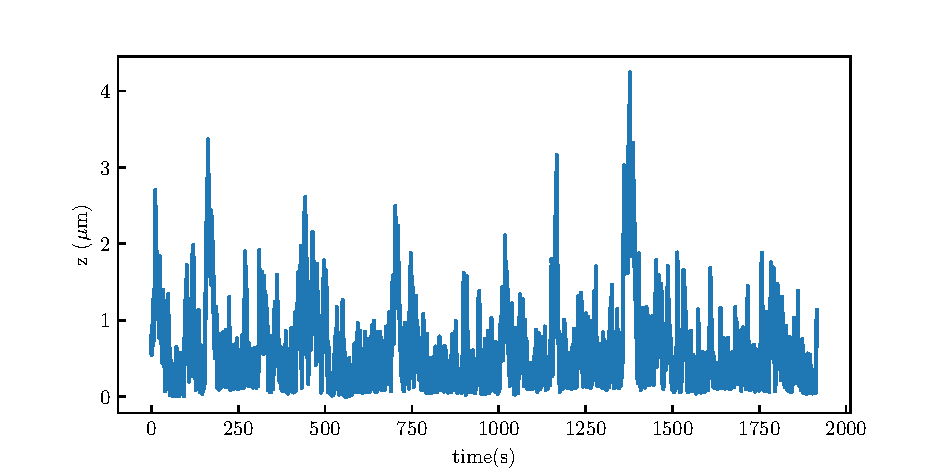
\includegraphics{02_body/chapter3/images/traj_z/traj_z.pdf}
	\caption{Experimental trajectory of a polystyrene particle of radius $a = 1.5 ~ \mathrm{\mu m}$ in water near a glass wall ($z = 0$) along the $z$-axis --- \textit{i.e} perpendicular to the wall. \href{https://github.com/eXpensia/Confined-Brownian-Motion/blob/main/02_body/chapter3/images/traj_z/graph_ploting.ipynb}{\faGithub}}
	\label{Fig:exp_z_traj}
\end{figure}

\subsubsection{Gravitational potential}
\label{sec:gravit}


The density $\rho_\mathrm{p}$ of an observed colloid is different from the medium density $\rho_\mathrm{m}$. In our experiment, we used water whose density is $\rho_\mathrm{m} = 1000 ~ \mathrm{kg.m^{-3}}$. Thus, the particles are subject to gravitational potential given by:

\begin{equation}
	U_\mathrm{g} (z) = \Delta m g z = \frac{4}{3}\pi a ^3 g \Delta \rho z ~,
	\label{eq:ug_full}
\end{equation}

where $\Delta m$ is the difference between the mass of the particle and that of a fluid sphere of the same size, $\Delta \rho = \rho_\mathrm{m} - \rho_\mathrm{p}$ is the corresponding density difference, and $g$ is the gravitational acceleration. By invoking the definition of the Boltzmann length:

\begin{equation}
	\ell _\mathrm{B} = \frac{k_\mathrm{B}T}{(4/3) \pi a ^3 \Delta \rho g } ~,
\end{equation}

one can rewrite Eq.~(\ref{eq:ug_full}) as:

\begin{equation}
	U_\mathrm{g}(z) = \frac{k_\mathrm{B}T}{\ell _\mathrm{B}}z ~.
	\label{eq:ug}
\end{equation}

The Boltzmann length $\ell_\mathrm{B}$ corresponds to the spatial extent over which the change of gravitational energy equals thermal energy. This distance was first measured by Perrin \cite{perrin_les_2014}. To do so, using a microscope he counted the number of colloidal particles as a function of the height in the sample. Then, he reconstructed the concentration profile of the colloidal suspension that exponentially decays as $\mathrm{e}^{- z / \ell _\mathrm{B}}$. As an example, for a polystyrene particle of radius $a  = 1.5 ~ \mathrm{\mu m}$ in water, one has $\ell _\mathrm{B} = 580 ~ \mathrm{nm}$.

For systems with $\ell _\mathrm{B} >> h $, where $h$ is the vertical thickness of the sample, one can consider that the particle does not feel gravity. This is particularly the case when the densities of the colloids and the fluid are equal. In this particular case, one has $\ell _\mathrm{B} = \infty$. Thus, density matching can be a way to do gravity-free experiments. In our experiment, we want to measure confinement-induced effects. Therefore, we need gravity for particles to be driven towards the substrate. As particles get larger or denser, $\ell _\mathrm{B}$ decreases and particles are, on average, closer to the substrate. 


\subsubsection{Sphere-wall interactions}
\label{Section:sphere-wall}



As we have seen, external forces such as gravity act on the particles. As Brownian particles are close to a wall, we can also expect some interactions between the particles and the wall. In our case, we suppose that the Brownian particles do not interact with each other, as we consider dilute solutions only. Indeed, the studied particles are at least $50 ~ \mathrm{\mu m}$ apart from each other, which corresponds to 10 times their size for the largest beads. 

To describe the interaction between a Brownian particle and the wall, we use the DLVO theory, named after Derjaguin, Landau, Verwey, and Overbeek \cite{israelachvili_intermolecular_2015}. This theory was first developed to describe the interactions between colloids, and explains the stability of colloidal suspensions. It involves two force components; the Hamaker force which arises from van der Waals interactions between the molecules of the two surfaces and a screened electrostatic force due to a double layer of charges formed near each surface, and involving the ions present in the solution. 

\paragraph{Double layer interactions}\mbox{}\\
\label{subsec:double}
\vspace{0.10cm}


When a surface is immersed in water, it usually acquire charges \cite{israelachvili_intermolecular_2015} due to a high water dielectric constant $\epsilon = \epsilon_0 \epsilon_\mathrm{r}$, where $\epsilon_0$ is the vacuum permittivity and $\epsilon_\mathrm{r}$ the medium relative permittivity; for water $\epsilon_\mathrm{r} = 80$. Commonly, surface charging is done through the ionization of  surface groups\footnote{For example, the dissociation of protons from surface carboxylic groups \cite{israelachvili_intermolecular_2015} ($-$COOH $\rightarrow$ -COO$^-$ + H$^+$) which charges negatively the surface.}, or from the binding of ions from the solution --- for example, adsorption of $-$OH$^-$ onto the water-air interface that charges it negatively. In the bulk, a fluid is electrically neutral; thus the fluid contains as equal number of ions of opposite charges (including the proper stoichiometry due to ionic valencies). However, when a surface is negatively charged, the negative ions are repelled from it, while positive ions are attracted towards it.  Therefore, a double-layer charge distribution is formed near the surface, as shown in Fig.~\ref{Fig:double_layer}. Experimentally, we use glass slides and polystyrene beads that are both negatively charged in water leading to a repulsive interaction between them. This repulsive force prevents the colloids from sticking together, or to the substrate's surface.

The DLVO theory states that the electrostatic potential $\Psi(\vec{r})$ generated by an ion of one given species $i$ at a distance $\vec{r}$ satisfies the Poisson equation \cite{israelachvili_intermolecular_2015}:

\begin{equation}
	\nabla ^2 \Psi(\vec{r}) = -\frac{1}{\epsilon_\mathrm{r} \epsilon_0}  \rho_\mathrm{e}(\vec{r})~,
	\label{Eq:poisson}
\end{equation}

with:

\begin{equation}
	\rho_\mathrm{e}(\vec{r}) = e \sum _i z_i c_i (\vec{r}) ~,
	\label{Eq.3}
\end{equation}

\begin{figure}
	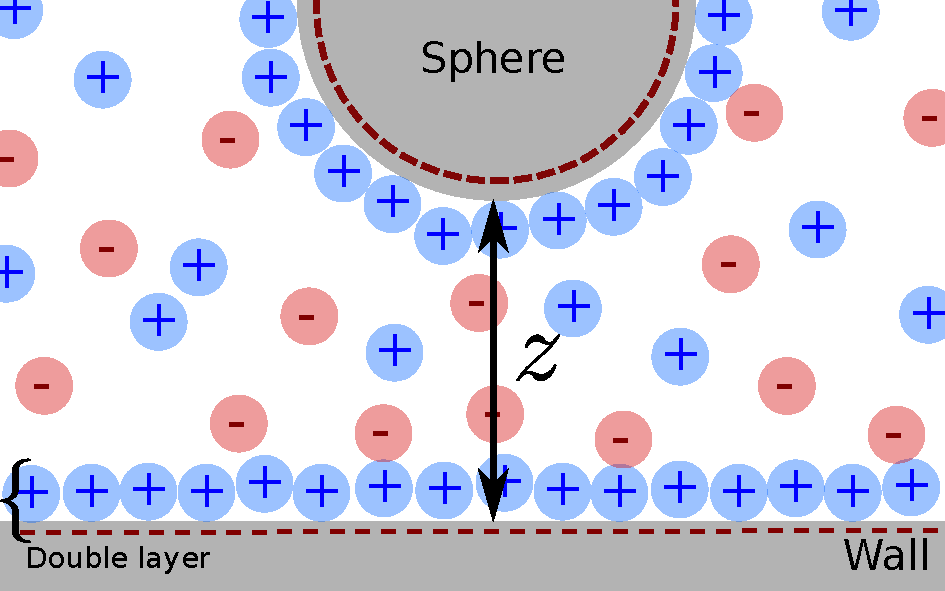
\includegraphics{02_body/chapter3/images/double_layer.pdf}
	\caption{A colloid diffusing near a wall. Both the wall and colloid surfaces charge negatively. As a consequence, a layer of positively-charged ions is attracted towards each surface, forming a double layer.}
	\label{Fig:double_layer}
\end{figure}


the local charge density, where $e$ is the elementary charge, and where the index $i$ denotes an ionic species of valence $z_i$ and local ionic concentration $c_i$ (number density). If the solution is at thermodynamic equilibrium, the local ionic density is given by a Gibbs-Boltzmann distribution, as:

\begin{equation}
	c_i(\vec{r}) = c_i ^0 \textnormal{exp}\left(\frac{-z_i e \Psi(\vec{r})}{k_\mathrm{B} T }\right) ~,
	\label{Eq.4}
\end{equation}


where $c_i ^0$ is the bulk concentration (number density) of the ionic species $i$. By combining Eqs.~(\ref{Eq:poisson}),~(\ref{Eq.3})~and~(\ref{Eq.4}), one obtains the Poisson-Boltzmann equation:

\begin{equation}
	\nabla ^2 \Psi (\vec{r}) + \sum_i \frac{z_i e c_i^0}{\epsilon_0 \epsilon_\mathrm{r}} \exp \left( - \frac{z_i e \Psi (\vec{r})}{k_\mathrm{B}T} \right) = 0 ~.
	\label{Eq:Poisson-boltzmann}
\end{equation}

Since Eq.~(\ref{Eq:Poisson-boltzmann}) is nonlinear, it is typically solved numerically. However, for some simple configurations such as uniformly-charged plane or sphere it can be solved analytically. To simplify, let us consider that we have a monovalent electrolyte, meaning that the electrolyte is composed of two ions of valencies both equal to 1 --- Na$^+$ Cl$^-$ for example --- and $c_i ^0$ is equal to the bulk electrolytic concentration $c_s^0$. In such a case, Eq.~(\ref{Eq:Poisson-boltzmann}) simplifies and becomes:

\begin{equation}
	\begin{aligned}
		&\nabla ^2 \Psi (\vec{r}) + \frac{e c_s ^0}{\epsilon_0 \epsilon_\mathrm{r}} \left[ \exp \left( \frac{-e\Psi(\vec{r})}{k_\mathrm{B}T} \right) -  \exp \left( \frac{+e\Psi(\vec{r})}{k_\mathrm{B}T} \right) \right] = 0 \\
		&\nabla ^2 \Psi (\vec{r}) + 2 \frac{e c_s ^0}{\epsilon_0 \epsilon_\mathrm{r}} \mathrm{sinh}  \left( \frac{e\Psi(\vec{r})}{k_\mathrm{B}T} \right) = 0 ~.
	\end{aligned}
\end{equation}


Another situation leading to analytical results, is when $\Psi$ is small enough such that $e\Psi \ll k_\mathrm{B} T$, which is generally the case when using dilute enough solutions, it is possible, through a Taylor expansion at first order to write:

\begin{equation}
	\exp \left( - \frac{z_i e \Psi(\vec{r})}{k_\mathrm{B}T} \right) \simeq 1 - \frac{z_i e \Psi (\vec{r})}{k_\mathrm{B}T} ~.
\end{equation}

In such case, Eq.~(\ref{Eq:Poisson-boltzmann}) becomes:

\begin{equation}
	\nabla ^2 \Psi (\vec{r}) + \sum_i \frac{z_i e c_i^0}{\epsilon_0 \epsilon_\mathrm{r}}  \left( 1 - \frac{z_i e \Psi (\vec{r})}{k_\mathrm{B}T} \right)  = 0~.
	\label{Eq:poisson_b_3}
\end{equation}

In addition, a fluid is electrically neutral. Therefore, $\sum_i z_i c_i^0 = 0$. Thus, one can simplify Eq.~(\ref{Eq:poisson_b_3}) to get the Debye-Hückel equation:

\begin{equation}
	\nabla^2 \Psi (\vec{r}) = \left[  \sum_i \frac{z_i ^2 e^2 c_i^0}{\epsilon_0 \epsilon_\mathrm{r}  k_\mathrm{B} T}    \right] \Psi (\vec{r}) ~.
	\label{debh1}
\end{equation}

One can identify the term between brackets as the inverse of a length squared. We thus define the Debye length as:

\begin{equation}
	\ell _\mathrm{D} =  \sqrt{ \sum_i\frac {\epsilon_0 \epsilon_\mathrm{r} k_\mathrm{B} T} {z_i ^2 e^2 c_i^0}} ~,
	\label{ld1}
\end{equation}

which is the characteristic ion-induced screening length of the electrostatic interactions, as we will see below. For a monovalent electrolyte,  at 25 \textdegree C, the Debye length of an aqueous solution is:

\begin{equation}
	\begin{aligned}
		\ell _\mathrm{D} &= \sqrt{\frac{ 2 \epsilon_0 \epsilon_\mathrm{r} k_\mathrm{B}T}{c_s^0 e^2}}
		& = \frac{0.304 }{ \sqrt{C} } ~\mathrm{nm} ~,
	\end{aligned}
	\label{ldnacl}
\end{equation}


with $C$ the value of the molar concentration in $\mathrm{mol.L^{-1}}$:

\begin{equation}
	C = \frac{c_\mathrm{s} ^0}{N_\mathrm{A}} 10^{-3} ~. 
\end{equation}


For example, for NaCl salt in water,  $\ell_\mathrm{D} \approx 100 ~ \mathrm{nm}$ for a concentration  $C = [\mathrm{NaCl}] = 9.2 ~ \mathrm{\mu mol.L^{-1}}$ and   $\ell_\mathrm{D} \approx 10 ~  \mathrm{nm}$ for a concentration  $[\mathrm{NaCl}] = 9.2 ~ \mathrm{mmol.L^{-1}}$.



Finally, combining Eqs.~(\ref{debh1})~and~(\ref{ld1}),  the Debye-Hückel equation reads:

\begin{equation}
	\nabla^2 \Psi (\vec{r}) = \kappa^2  \Psi (\vec{r}) ~,
	\label{Eq:Debye_hu}
\end{equation}

with $\kappa = 1/\ell _\mathrm{D}$. Using the latter, one can compute the electrostatic potential around a sphere immersed in an ionic solution. Let us consider a sphere of radius $a$ and charge $Qe$, \textit{i.e.} a charge density $\sigma = Qe/(4\pi a^2)$ , $Q$ being the number of charges on the surface. Since the system has a spherical symmetry, one has $\Psi (\vec{r}) = \Psi(r)$ with $r = |\vec{r}|$. Using the Laplacian operator $\nabla ^2$ in spherical coordinates, Eq.~(\ref{Eq:Debye_hu}) becomes:

\begin{equation}
	\frac{1}{r^2}\left[\frac{\partial}{\partial r} \left(r^2 \frac{\partial \Psi(r)}{\partial r}\right)\right] = \kappa^2  \Psi (r) ~,
\end{equation}

which has a general solution:

\begin{equation}
	\Psi(r) = C_1 \frac{\exp(\kappa r)}{r} + C_2 \frac{\exp(-\kappa r)}{r}~.
\end{equation}

The electrostatic potential vanishes at infinity such that $C_1 = 0$. Therefore, the electrostatic potential (and thus the electrostatic energy potential) takes the form of a Yukawa potential:

\begin{equation}
	\Psi (r) = C_2 \frac{\exp(-\kappa r)}{r} ~.
	\label{eq:yuka}
\end{equation}

Additionally, invoking the Gauss theorem, at the surface of the charged sphere, the electrostatic potential satisfies:

\begin{equation}
	\left. \frac{\partial{\Psi (r)}}{\partial r} \right|_{r=a} = \frac{-Qe}{4 \pi \epsilon_0 \epsilon_\mathrm{r} a^2}  = \frac{-\sigma}{\epsilon_0 \epsilon_\mathrm{r}} ~,
\end{equation}

where we introduced the surface density of charges $\sigma$. By applying the latter boundary condition to Eq.~(\ref{eq:yuka}), we find:

\begin{equation}
	\Psi (r) = \frac{\sigma a^2}{\epsilon_0 \epsilon_\mathrm{r}} \frac{\exp (\kappa a)}{1 + \kappa a} \frac{\exp (-\kappa r)}{r} ~.
\end{equation}

This solution can be used to determine the electrostatic potential between two spheres of radii $a_1$ and $a_2$, and surface charge densities $\sigma_1$ and $\sigma_2$, respectively. Supposing that the presence of a second sphere does not modify the distribution of ions in the double layer of the other sphere, one can use the superposition approximation to obtain the potential $U_\textrm{elec} ^{ss} (z)$ between the two spheres \cite{bell_approximate_1970}:

\begin{equation}
	U_\textrm{elec} ^{ss}(z) = \frac{4\pi}{\epsilon_0 \epsilon_\mathrm{r}} 
	\left(
	\frac{\sigma_1 a_1 ^2}{1 + \kappa a_1}
	\right)
	\left(
	\frac{\sigma_2 a_2 ^2}{1 + \kappa a_2}
	\right)
	\frac{\exp(-\kappa z)}{a_1 + a_2 + z} ~,
\end{equation} 
with $z$ the gap between the two colloids.
From the latter equation, it is possible to write the electrostatic interaction energy $U_\textrm{elec}$ between a planar wall of charge density $\sigma_\textrm{w}$ and a spherical colloid of radius $a$ and surface charge density $\sigma$, by setting one of the two radii to infinity. Doing so, one gets:

\begin{equation}
	\frac{U_\textrm{elec}(z)}{k_\mathrm{B}T}  = B \mathrm{e}^{-\frac{z}{\ell_\mathrm{D}}}~,
	\label{Eq:Uelec}
\end{equation}

where:

\begin{equation}
	B = \frac{4 \pi}{ k_\mathrm{B}T\epsilon_0 \epsilon_\mathrm{r}} \left( \frac{\sigma a^2 }{1 + \kappa a}  \right) \frac{\sigma_\mathrm{w}}{\kappa} ~.
\end{equation}

Let us note that, $B$ is often written as \cite{behrens_charge_2001}:

\begin{equation}
	B = 16 \epsilon_\mathrm{r} \epsilon_0 a \frac{ k_\mathrm{B}T }{e^2} \tanh \left(\frac{e\phi}{4k_\mathrm{B}T}\right) \tanh \left(\frac{e\phi_\mathrm{w}}{4k_\mathrm{B}T}\right) ~,
\end{equation}
where $\phi$ and $\phi_\mathrm{w}$ are the Stern potentials of the sphere and wall surface, respectively. Typical values for $B$ range from 1 to 50. In our study, we will use $B$  to characterize the dimensionless magnitude of the electrostatic interaction. Indeed, it ois complicated to decouple $\sigma$ and $\sigma_\mathrm{w}$ when the colloid and wall materials are different \cite{behrens_charge_2001}.

\paragraph{van der Waals interactions}\mbox{}\\
\vspace{0.10cm}

\begin{figure}[h]
	\centering
	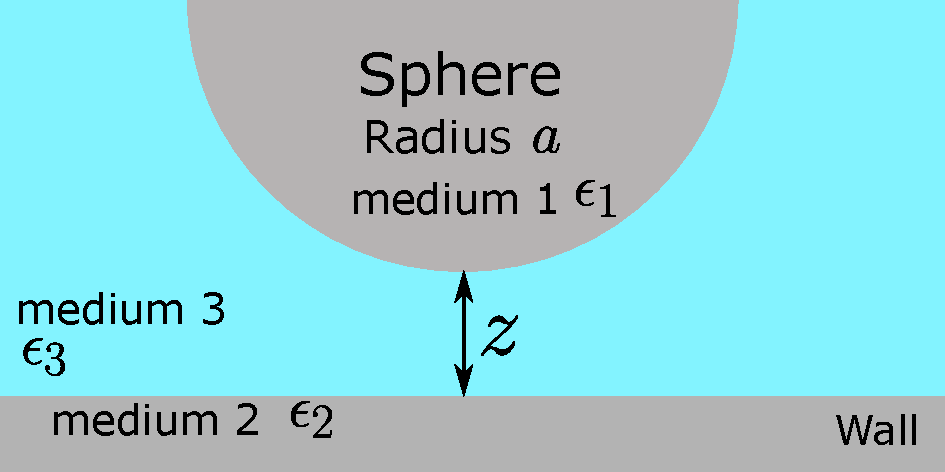
\includegraphics{02_body/chapter3/images/vdw_scheme.pdf}
	\caption{A colloid of radius $a$ is located at a distance $z$ from the wall. The dielectric constants of the sphere, wall and liquid are respectively $\epsilon_1$, $\epsilon_2$, and $\epsilon_3$. }
	\label{Fig:vdw}
\end{figure}

In the DLVO theory, van der Waals interactions, after integration over all surfaces contribute through a global Hamaker potential energy. This potential is short-ranged and attractive, in our case.The interaction potential reads: \cite{israelachvili_intermolecular_2015}:

\begin{equation}
	U_\mathrm{vdW} = -\frac{A a}{6z} 
\end{equation}

where $A$ is the nonretarded Hamaker constant. For our system, where the particle, medium and wall are different media as schematize in Fig.~\ref{Fig:vdw}, the Hamaker constant is given by \cite{israelachvili_intermolecular_2015}:

\begin{equation}
	A = \frac{3}{4} k_\mathrm{B}T \left(
	\frac{\epsilon_1 - \epsilon_3}{\epsilon_1 + \epsilon_3}
	\right)
	\left(
	\frac{\epsilon_2 - \epsilon_3}{\epsilon_2 + \epsilon_3}
	\right)
	+
	\frac{3h}{4\pi}
	\int_{\nu_1}^{\infty}
	\left(
	\frac{\epsilon_1 (j\nu) - \epsilon_3 (j\nu)}{\epsilon_1 (j\nu) + \epsilon_3 (j\nu)}
	\right)
	\left(
	\frac{\epsilon_2 (j\nu) - \epsilon_3 (j\nu)}{\epsilon_2 (j\nu) + \epsilon_3 (j\nu)}
	\right)
	\textnormal{d}\nu ~,
\end{equation}

where $\epsilon_1$, $\epsilon_2$ and $\epsilon_3$ are the static dielectric constants of the three media, $\epsilon_{1,2,3} (j\nu)$ are the  dielectric constant at a imaginary frequency $ j \nu$. The first term gives the zero-frequency energy of the Van der Waals interaction and the second term the dispersion energy. In the literature, we found for polystyrene colloids in water near a glass substrate $A\approx k_\mathrm{B}T$. Since $A$ is positive, the interaction is attractive, moreover, we estimate that the van der Waals forces play a role only within a few nanometers from the surface ($z < 10$ nm), as commonly observed \cite{prieve_measurement_1999}. In our experiments, the Debye length $\ell _\mathrm{D}$ ($>20$ nm) is large enough for the particles to avoid this region. Therefore, in the following, the van der Waals interactions are neglected. It is possible to study the van der Waals interactions with Brownian motion, provided that one adds enough salt to have $\ell_\mathrm{D} \simeq 1$ nm. However, with such a short Debye length, all the colloids would stick to the surface and with each other, as a result of van der Waals forces. Interestingly, we have experimentally observed stuck particles. Further work on these events may lead to interesting insights about of the near-wall interactions. 



\paragraph{Total potential and equilibrium distribution}\mbox{}\\
\label{test}
\vspace{0.10cm}

If we combine the gravitational and electrostatic energy potentials the particles lie into a total energy potential $U(z)$, given by:

\begin{equation}
	U(z) = U_\mathrm{g} + U_\mathrm{elec}~.
	\label{eq:uz}
\end{equation}

By combining Eqs.~(\ref{eq:ug}),~(\ref{Eq:Uelec})~and~(\ref{eq:uz}), and adding the condition that a particle cannot go inside the wall, one finally gets:

\begin{equation}
	\frac{U(z)}{k_\mathrm{B}T} =  \left\{
	\begin{array}{l}
		\displaystyle B\,\textrm{e}^{-\frac{z}{\ell_\mathrm{D}}} + \frac{z}{\ell_\mathrm{B}}\ ,\quad \text{ for } z>0 \\
		+\infty\ ,\quad  \text{ for } z < 0
	\end{array}
	\right. \ .
	\label{Eq:PDF}
\end{equation}

From this total potential energy, one can then construct the Gibbs-Boltzmann distribution to write the equilibrium \gls{PDF} of position $P_{\mathrm{eq}}(z)$:

\begin{equation}
	P_\mathrm{eq} (z)  = A \exp \left( -\frac{U(z)}{k_\mathrm{B}T} \right) ~,
	\label{Eq.Peq}
\end{equation} 

where $A$ is a normalization constant such that $\int_{0}^{\infty}P_\mathrm{eq}(z)\textnormal{d}z = 1$. Given an ensemble of heights $z_i$, one can compute $P_\mathrm{eq}$ using the following Python function \mintinline{python}{Peq}, where the $A$ is computed using the \mintinline{python}{np.trapz} function. Examples of a theoretical energy potential and associated \gls{PDF} of position can be seen in Fig.~\ref{Fig:potential} for $\ell_\mathrm{B} = 500 ~ \mathrm{nm} $,  $B = 4$ and $\ell_\mathrm{D} = 50 ~ \mathrm{nm}$.


\begin{minted}
	[
	autogobble,
	frame=lines,
	framesep=2mm,
	baselinestretch=1.2,
	obeytabs=true,
	tabsize=2,
	fontsize=\footnotesize,
	linenos
	]
	{python}
import numpy as np
	
def _Peq(z):
	if z <= 0:
		return 0
	else:
		return np.exp(-(B * np.exp(-z / ld) + z / lb))
	
	
def Peq(z):
	P = np.array([_Peq(zi) for zi in z])
return P / np.trapz(P,z)
\end{minted}

\begin{figure}[h]
	\centering
	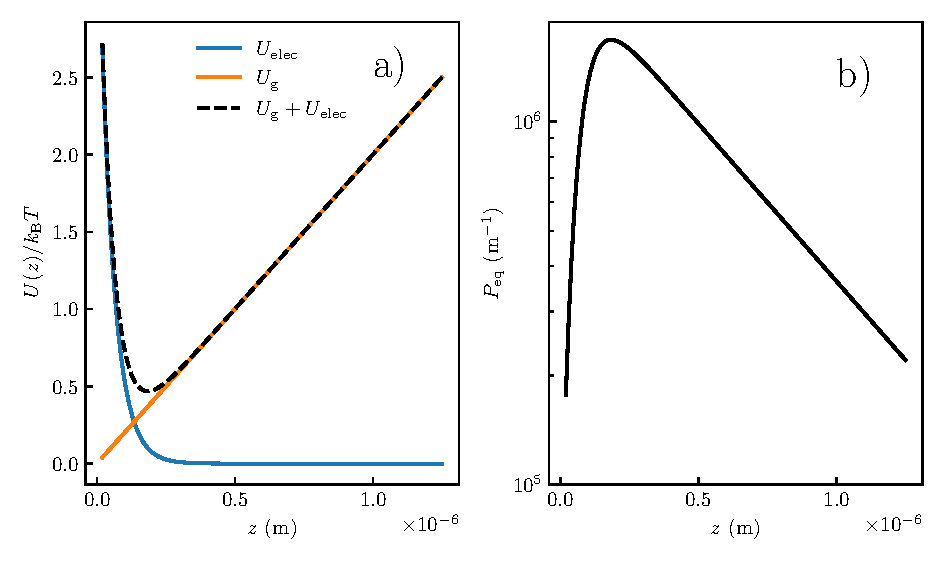
\includegraphics{02_body/chapter3/images/potential/potential_exemple.pdf}
	\caption{ a) In orange potential energy $U_\mathrm{g}$ (see Eq.~(\ref{eq:ug})) of a colloid with a Boltzmann length $\ell_\mathrm{B} = 500 ~ \mathrm{nm} $. In blue, the electrostatic potential energy $U_\mathrm{elec}$ (see Eq.~(\ref{Eq:Uelec})) is characterized by a dimensionless magnitude $B = 4$ and a Debye length $\ell_\mathrm{D} = 50 ~ \mathrm{nm}$. The dashed line corresponds to the total potential $U$, see Eq.~(\ref{eq:uz}). b) Corresponding Gibbs-Boltzmann equilibrium distribution of position calculated using the energy potential of panel a). \href{https://github.com/eXpensia/Confined-Brownian-Motion/blob/main/02_body/chapter3/images/potential/potential_exemple.ipynb}{\faGithub}}
	\label{Fig:potential}
\end{figure}

\newpage

\subsubsection{Local diffusion coefficient}
\label{sec:diff}
\begin{figure}
	\centering
	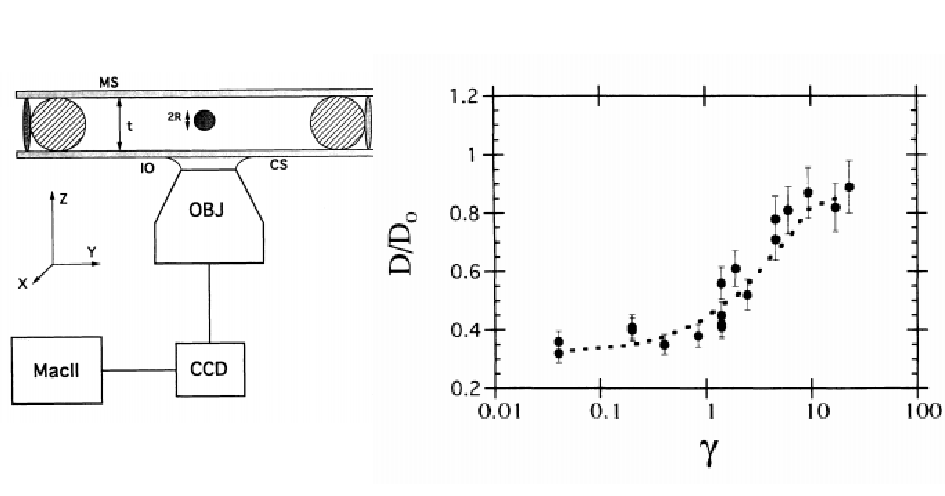
\includegraphics{02_body/chapter1/image/libchaber.pdf}
	\caption{Figure extracted from \cite{faucheux_confined_1994}. On the left is the experimental setup. It is an inverted microscope used in order to track micrometric particles of diameter $2R$ inside a liquid cell of thickness $t$. On the right is the final result, where the authors measure the diffusion parallel (\textit{i.e.} along $x$ or $y$) coefficient $D_\parallel$ (see Eqs.~(\ref{Eq:etax})~and~(\ref{Eq.hindered})), normalized by the bulk diffusion coefficient $D_0$, as a function the confinement parameter $\gamma = \langle z \rangle_t/a$, with $\langle z \rangle_t$ time-averaged particle-wall distance.}
	\label{fig:libchaber}
\end{figure}


As we have seen in Chapter~\ref{sec:chapter1}, for a freely diffusing colloid in the bulk, the diffusion coefficient is given by Eq.~(\ref{Eq:D_einstein}) and is a constant. However, when a particle is confined by a rigid wall, the diffusion is hindered. This means that the diffusion coefficient varies with the particle-wall distance and becomes anisotropic.A seminal measurement of this effect was done by Faucheux and Libchaber \cite{faucheux_confined_1994}. As we can see in Fig.~\ref{fig:libchaber}, using a microscope, they tracked colloids within a parallelepipedic chamber, and measured the thickness-averaged diffusion coefficients for different values of the confinement parameter $\gamma = \langle z\rangle_t / a$, with $\langle z \rangle_t$ time-averaged particle-wall distance. As experiments reach equilibrium, $\langle z \rangle_t$ is given by the Gibbs-Boltzmann distribution as $\langle z \rangle_t = \int \textnormal{d}zP_\mathrm{eq}(z))z$. We observe that the diffusion coefficient parallel to the surface decreases as the particle gets closer to the wall, and seems to saturate around $0.3D_0$ at low $\gamma$, with $D_0$ the diffusion coefficient in the bulk (see Eq.~\ref{Eq.D}). 
\newpage

To understand the reason for this hindered diffusion coefficient, let us start by writing the diffusion coefficient $D$ using the fluctuation dissipation theorem:

\begin{equation}
	D = \frac{1}{\gamma} k_\mathrm{B}T ~,
	\label{Eq.fluc}
\end{equation}

with the mobility defined as:

\begin{equation}
	\frac{1}{\gamma} = \left| \frac{v_\mathrm{sphere}}{F_\mathrm{drag}} \right|~,
	\label{Eq.mu}
\end{equation}

where $v_\mathrm{sphere}$ is the terminal velocity to an applied force $F_\mathrm{drag}$. For a spherical colloid of radius $a$ moving at a velocity $v_\mathrm{sphere}$, the drag force $F_{\mathrm{drag}} ^\mathrm{B}$ is given by the Stokes' law:

\begin{equation}
	F_\mathrm{drag} ^\mathrm{B} = -c \pi \eta a v_\mathrm{sphere} ~,
	\label{Eq.drag}
\end{equation}

where $c$ is a constant that depends on the boundary conditions imposed at the surface of the colloid. Typically, one has $c = 6$ for a no-slip boundary conditions and $c = 4$ for a full-slip boundary conditions, such as for air bubbles, for example. Combining Eqs.~(\ref{Eq.fluc}),~(\ref{Eq.mu})~and~(\ref{Eq.drag}) for a freely diffusing no-slip hard sphere in the bulk we retrieve Eq.~(\ref{Eq:D_einstein}): 

\begin{equation}
	D = D_0 = \frac{k_\mathrm{B}T}{6\pi \eta a} ~.
	\label{Eq.D}
\end{equation}

The Stokes' drag force can be computed by solving the Navier-Stokes equation:

\begin{equation}
	\rho \left[ \frac{\partial \vec{v}}{\partial t} + \left(\vec{v} \cdot \nabla \vec{v} \right) \right] + \nabla p = \eta \nabla ^2 \vec{v} ~,
	\label{Eq.Navier}
\end{equation}

and the continuity equation for incompressible fluids:

\begin{equation}
	\nabla \cdot \vec{v} = 0~,
	\label{Eq.continuity}
\end{equation}

where $\vec{v}$ and $p$ are receptively the velocity and pressure fields, and where $\rho$ is the liquid density. When the Reynolds number $\textnormal{Re} = \rho a v_\mathrm{sphere} / \eta \ll 1$,  the second inertial term is negligibly small compared to the viscous term $\eta \nabla ^2 \vec{v}$. In that case, and at long-enough time for the first inertial term to be negligible, the Eq.~(\ref{Eq.Navier}) is simplified to the steady Stokes equation:

\begin{equation}
	\nabla p = \eta \nabla ^2 \vec{v}~.
	\label{Eq.Stokesflow}
\end{equation}

By solving Eqs.~(\ref{Eq.continuity})~and~(\ref{Eq.Stokesflow}) with a no-slip boundary condition on the particle surface and the field vanishing at infinity, one can calculate the velocity and the pressure fields in the fluid. By integration of the pressure and viscous stress on the particle surface, one eventually gets the Stokes mobility. However, in the case of a confined particle near a wall there is an additional no-slip condition at the wall surface. At the macro scale, this effect can be seen with a frisbee, indeed, as it gets closer to the ground, hydrodynamic pressure increases due to the increasing air velocity gradient in the gap and one can observe a slowing down of the free fall.

To get some physical insight on this effect, one can use the lubrication theory to make a scaling of the drag force experience by a particle confined near a wall. As schematized in Fig.~\ref{fig.shear}, we consider a particle of radius $a$ moving at a velocity $V$. 

\begin{figure}[ht]
	\centering
	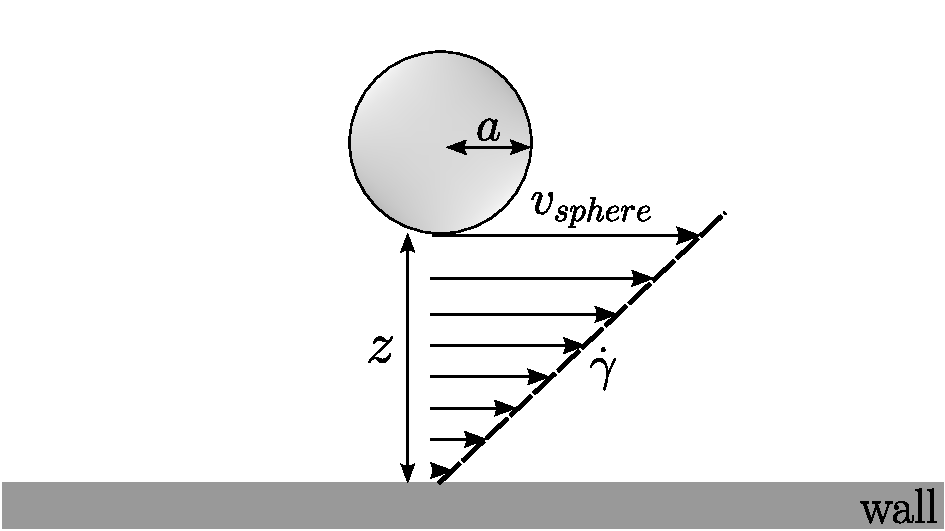
\includegraphics{02_body/chapter3/images/draw_shear/shear.pdf}
	\caption{Schematic representation of a spherical object of radius $a$ moving towards a wall at velocity $V_\mathrm{sphere}$ and inducing a fluid velocity $V_\mathrm{fluid}$} 
	\label{fig.shear}
\end{figure}

As we are using the lubrication theory, we suppose that the particle is close to the wall such that $h \ll a$. In that condition, we suppose that a particle moving towards a wall (\textit{along the $z$-axis}) at a velocity $V_\mathrm{sphere}$ induce a fluid velocity $V_\mathrm{fluid}$ along the $x$-axis, we further suppose that the induced velocity along the $z$-axis is negligible. Moreover, the typical length scale along the $z$-axis is the particle-wall distance $z$; and the distance $L=\sqrt{az}$ (\textit{i.e.} Hertz contact), along the $x$-axis. In this approximation, velocity terms along the $z$-axis will be negligible in Eq.~(\ref{Eq.Stokesflow}), a projection along the $z$-axis thus gives:

\begin{equation}
	\frac{\partial p}{\partial z} = 0 ~.
\end{equation}

On the right-hand side of Eq.~\ref{Eq.Stokesflow}, the viscous term simplifies to $\eta \partial_z^2 V_\mathrm{fluid} $ as:

\begin{equation}
	\frac{\partial^2 V_\mathrm{fluid}}{\partial x^2} \approx \frac{V_\mathrm{fluid}}{L^2} \ll \frac{V_\mathrm{fluid}}{h^2} \approx \frac{\partial^2 V_\mathrm{fluid}}{\partial z^2}~.
\end{equation}

In the lubrication theory, Eq.~(\ref{Eq.Stokesflow}) is finally simplified to:

\begin{equation}
	\frac{\partial p}{\partial x} = \eta \frac{\partial ^2 V_\mathrm{fluid}}{\partial z^2}~.
\end{equation}

By replacing the partial derivative by the typical length leads to:

\begin{equation}
	p \sim \eta V_\mathrm{fluid} \frac{L}{z^2}
	\label{pressure}
\end{equation}

To compute the calculate the Stokes mobility, one needs to evaluate the viscous stress $\sigma$, in the lubrication theory, it reads:

\begin{equation}
	\sigma = \eta \frac{\partial V_\mathrm{fluid}}{\partial z} \sim \eta \frac{V_\mathrm{fluid}}{h}
\end{equation}

When the particle is moving towards the wall we thus have $p\gg \sigma$, we thus only consider the pressure. To evaluate the mobility, we need to write Eq.~(\ref{pressure}) as a function of $V_\mathrm{sphere}$. Using Eq.~(\ref{Eq.continuity}) equation one has $V_\mathrm{fluid} / h \sim  V_\mathrm{sphere} / L$, Eq.~(\ref{pressure}) thus become:

\begin{equation}
	p \sim \eta  \frac{L^4}{h^2}
\end{equation}

Integrating this pressure over the particle surface (\textit{i.e} over the typical length $L = \sqrt{az}$) leads a scaling of the drag force:

\begin{equation}
	F_\mathrm{drag} ^{z\ll a} \sim \eta V \frac{L^4}{h^2} = \eta V \frac{a^2}{z}
\end{equation}

The mobility (see Eq.~(\ref{Eq.mu})) of the displacement perpendicular to the wall  thus scale as $\gamma_0^{-1} h/a$, with $\gamma_0^{-1}$ the bulk mobility. Therefore, the diffusion coefficient of a confined colloid near a wall in the lubrication approximation is hindered and inversely proportional to the particle-wall distance. It is possible to same scaling for the parallel mobility by supposing that the particle is moving along the $x$-axis. In that case, one can find that the viscous stress is greater than the pressure and finally find that along the $x$-axis, the parallel mobility follows the same scaling as in bulk and remain constant.

To recap, a colloid diffusing near a wall thus experience a local drag force that depends on both its distance $z$ to the wall and direction of motion. Thanks to the linearity of the Stokes equation, one can decompose this local drag force in two contributions, for motions parallel and perpendicular to the wall. As the presence of the wall modifies the drag force with a space-dependent multiplicative factor, the confinement effect is often expressed in terms of effective viscosities:

\begin{equation}
	\eta _\bot (z) = {\eta}{\lambda _ \bot (z)}  ~ \text{, and } ~\eta _\parallel (z) =  {\eta}{\lambda _ \parallel (z)}~,
\end{equation}

where $\lambda _\bot$ and $\lambda _\parallel$ are respectively the perpendicular and parallel correction factors. Taking into account these corrections, the diffusion coefficients for perpendicular and parallel motions relative to the wall read:

\begin{equation}
	D_\bot (z) =  \frac{D_0}{\lambda _\bot (z)}  ~, \text{ and } D_\parallel (z) = \frac{D_0}{ \lambda_\parallel (z)} ~.
	\label{Eq.hindered}
\end{equation}

For no-slip boundary conditions imposed at both the wall and the surface of the colloid, Brenner \cite{brenner_slow_1961} obtained for the perpendicular motion:


\begin{equation}
	\lambda_ \bot (z) = \frac{4}{3}  \mathrm{sinh}\beta \sum _{n=1} ^{\infty} \frac{n(n+1)}{(2n-1)(2n+3)}
	\left[
	\frac
	{
		2\mathrm{sinh}(2n + 1)\beta + (2n +1)\mathrm{sinh}2\beta
	}
	{
		4\mathrm{sinh}^2(n + 1 /2)\beta  - (2n+1)^2 \mathrm{sinh}^2 \beta
	}
	-1
	\right] ~,
	\label{Eq:etaz}
\end{equation}

where $\beta = \cosh ^{-1} ((z+a)/a)$. For the motion of a sphere parallel to a wall, Faxén found \cite{faxen_fredholm_1924}:

\begin{equation}
	\lambda_\parallel(z) = 
	\left[
	1 - \frac{9}{16} \xi + \frac{1}{8}\xi^3 - \frac{45}{256}\xi^4 - \frac{1}{16}\xi^5
	\right]^{-1}~,
	\label{Eq:etax}
\end{equation}

where $\xi  = a / (z+a)$. Eqs.~(\ref{Eq:etaz})~and~(\ref{Eq:etax}) are exact for all $z$ and shown in Fig.~\ref{fig.etaz}-a). However, the solution for the perpendicular motion can be complex to compute as it is an infinite series. It requires a software that enables arbitrary-precision floating-point arithmetic\footnote{Arbitrary-precision floating-point arithmetic enables to evaluate mathematical expressions with any precision, \textit{i.e.} any number of digits.} --- such as Mathematica or the \mintinline{python}{mpmath} Python's module, for example. $D_\bot$ can be evaluated using the following Python snippet, where the \mintinline{python}|nsum| function is used to compute the summation:  
 
 \newpage


\begin{minted}
	[
	frame=lines,
	framesep=2mm,
	baselinestretch=1.2,
	fontsize=\footnotesize,
	linenos
	]
	{python}
from mpmath import nsum 
	
def Dz(eta, z, a):
  a = (z + a) / a
  beta = float(acosh(a))
  summ = nsum(
    lambda n: (n * (n + 1) / ((2 * n - 1) * (2 * n + 3)))
    * (
        (
          (2 * sinh((2 * n + 1) * xi) + (2 * n + 1) * sinh(2 * beta))
          / (
              4 * (sinh((n + 1 / 2) * beta) ** 2)
              - ((2 * n + 1) ** 2) * (sinh(beta) ** 2)
          )
    )
    - 1
  ),
  [0, inf],
  )
  summ = float(summ)
  return kT / (6 * pi * eta * 4 / 3 * float(sinh(beta)) * summ * a)

\end{minted}

To simplify the computation of $\lambda_\bot$, Honig \cite{honig_effect_1971}, and Bevan and Prieve \cite{bevan_hindered_2000} showed that Eq.~(\ref{Eq:etaz}) can be Padé approximated\footnote{A Padé aproximant is the approximation of a power series by a rational fraction \cite{baker_pade_1996}.}, giving:

\begin{equation}
	\lambda_\bot =  \frac{6z^2 + 9az + 2a^2}{6z^2 + 2az}~.
	\label{Eq:etaz_pade}
\end{equation}

In the near-wall regime, such that $z \ll a$, it is possible to further approximate $\lambda_\bot$ by its asymptotic expression:

\begin{equation}
	\lambda_\bot \simeq \frac{a}{z} ~.
	\label{Eq:etaz_small}
\end{equation}


\begin{figure}[H]
	\centering
	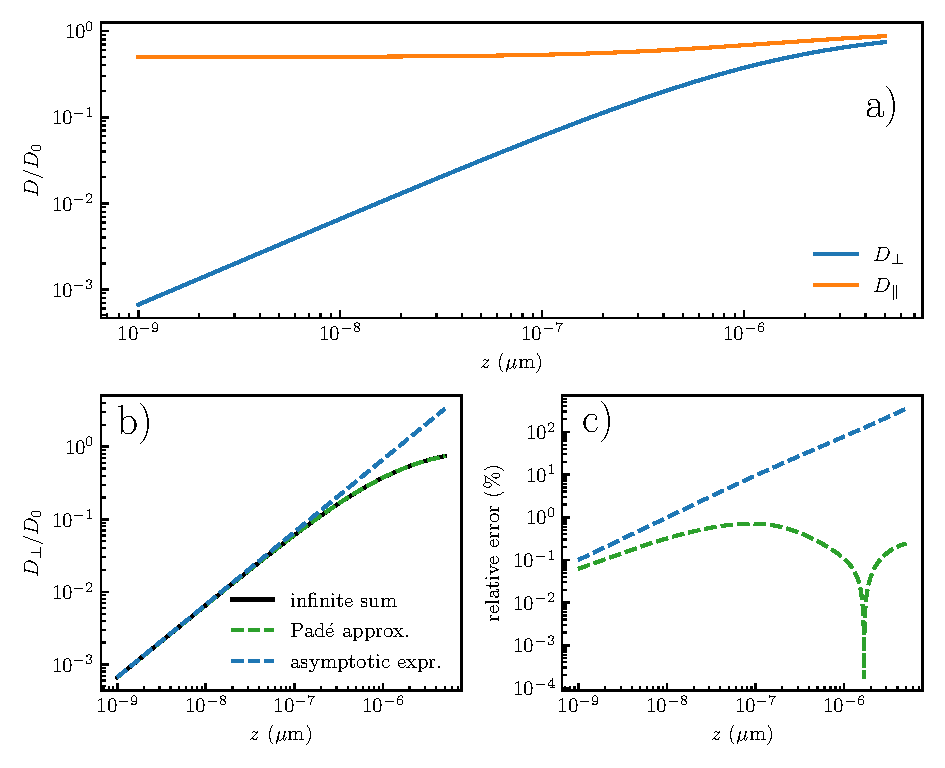
\includegraphics{02_body/chapter3/images/theory_lambda/hindered_diffusion.pdf}
	\caption{a)  Parallel and perpendicular normalized diffusion coefficients for a colloidal particle of radius $a = 1.5 ~ \mathrm{\mu m}$. b) Perpendicular normalized diffusion coefficient at a distance $z$ from a wall. The solid black line is the exact solution given by the infinite sum of Eq.~(\ref{Eq:etaz}). The green dashed line is the Padé approximation of Eq.~(\ref{Eq:etaz_pade}). The blue dahed line is the near-wall asymptotic expression of Eq.~(\ref{Eq:etaz_small}). c) Relative errors between the two approximations (dashed lines of panel b), same color code) and the exact result (solid line of panel b)).\href{https://github.com/eXpensia/Confined-Brownian-Motion/blob/main/02_body/chapter3/images/theory_lambda/Hindered_diffusion.ipynb}{\faGithub}}
	\label{fig.etaz}
\end{figure}


The exact result, together with the Padé approximation and the near-wall asymptotic expression for the hindered vertical diffusion are plotted in Fig.~\ref{fig.etaz}-b). The Padé approximation fits well the exact solution, the near-wall asymptotic expression fits well when $z < a / 10$ typically. To check how precise both approximations are, we plot the relative error in Fig.~\ref{fig.etaz}-c). The Padé approximation shows precision up to 1\%. Thus, in the following, when evaluating perpendicular diffusion coefficients, or equivalently vertical effective viscosities, the Padé approximation will be used. 


%\subsubsection{Langevin equation for confined Brownian motion}
%
%Now that the external forces acting on the particle and hindered diffusion coefficients are known, we rewrite the overdamped Langevin (see Eq.~(\ref{Eq.overdamped_SDE})) as:
%
%\begin{equation}
%	V_t^i \textnormal{d}t  = -\mu(z)\frac{\partial U(z)}{\partial x_i}  \textnormal{d}t + \sqrt{2D_i (z)}  \textnormal{d}B_t ~,
%	\label{Eq:langevin_z}
%\end{equation}
%
%where $\mu(z) = 1/ (6 \pi \eta_i(z) a)$, and $i$ denotes one of the three spatial directions, $x,~ y$ and $z$, where the previously determined $\eta_\parallel$ or $D_\parallel$ corresponds to the $x$- and $y$-axes, while $\eta_\bot$ or $D_\bot$ corresponds to the $z$-axis, and $ \textnormal{d}B_t$ is a Gaussian-distributed satisfying $\langle \textnormal{d}B_t \rangle = 0$ and $\langle \textnormal{d}B_t ^2 \rangle = \textnormal{d}t$. As discussed previously, the potential energy $U$ only varies along the $z$-axis, an thus, the external force only acts on the particle along the $z$-axis while the particle diffuses freely along the $x$- and $y$-axes. 


\subsubsection{Fokker-Plank equation}

The Fokker-Plank equation is an alternative way to describe Brownian motion. Instead of explicitly calculating a Brownian trajectory by solving the Langevin equation, Fokker-Plank equation describes the Probability Density Function $P(X_t, X_0; t)$ in position. Where for simplicity we place ourselve in 1D, with $X_t$ denoting the particle position at a time $t$ and $X_0$ its initial ($t=0$) position. To derive the Fokker-Plank equation, let us start by taking a generic Langevin equation in 1D:

\begin{equation}
	\textnormal{d}X_t = u(X_t) \mathrm{d}t + g\textnormal{d}B_t ~,
	\label{SDE2}
\end{equation}

where $u(X_t)$ is the drift velocity due to external forces and $g$ is the magnitude of the random force. Let consider the average value of an arbitrary function $f(X_t)$ for a stochastic process obeying Eq.~(\ref{SDE2}), which started at position $x_0$ at time $t=0$. By definition, this ensemble average reads \cite{le_bellac_equilibrium_2004}:

\begin{equation}
	\langle f(X_t) \rangle = \int \textnormal{d}X_t ~ P(X_t, X_0 ; t) f(X_t) ~,
	\label{fokker1}
\end{equation}

with the initial condition that can be written as:

\begin{equation}
P(X_t, X_0; 0) = \delta (X_t - X_0) ~.
\end{equation}

We now expand $f$ at the first order in the time increment $\textnormal{d}t$ as:

\begin{equation}
	\begin{aligned}
		\left\langle \frac{\textnormal{d}f(X_t)}{\textnormal{d}t} \right\rangle_t  &\simeq \left\langle \frac{1}{\textnormal{d}t} \left( \frac{\partial f(X_t)}{\partial X_t} u(X_t) \textnormal{d}t + \frac{\partial f(X_t)}{\partial X_t} g \textnormal{d}B_t + \frac{1}{2} \frac{\partial^2 f(X_t)}{\partial X_t^2} g^2  \textnormal{d}B_t^2   \right) \right\rangle_t \\
		& =  \frac{1}{\textnormal{d}t} \left( \frac{\partial f(X_t)}{\partial X_t} u(X_t) \textnormal{d}t + \frac{1}{2} \frac{\partial^2 f(X_t)}{\partial X_t^2} g^2 \textnormal{d}t \right) \\
		& = \frac{\partial f(X_t)}{\partial X_t} u(X_t) + \frac{1}{2} g^2 \frac{\partial^2 f(X_t)}{\partial X_t^2}   ~.
	\end{aligned}
	\label{fokker2}
\end{equation}

By combining Eqs.~(\ref{fokker1})~and~(\ref{fokker2}), we get:

\begin{equation}
	\begin{aligned}
		\int \textnormal{d} X_t ~\frac{\partial P(X_t, X_0 ; t) }{\partial t} f(X_t)
		& =  \frac{\partial f(X_t)}{\partial X_t} u(X_t) + \frac{1}{2} \frac{\partial^2 f(X_t)}{\partial X_t^2} g^2 \\
		& = \int \textnormal{d}X_t ~ P(X_t, X_0 ; t) G f(X_t) ~,
	\end{aligned}
\end{equation}

where G is a differential operator called the generator and is defined by its action on a function $f$ as:

\begin{equation}
	Gf = \frac{1}{2} g^2 \frac{\partial ^2 f(X_t)}{\partial X_t^2} + u(X_t) \frac{\partial f(X_t)}{\partial X_t} ~.
\end{equation}

Using the definition of the adjoint of $G$, denoted $G ^\dagger$, one has:


\begin{equation}
	\begin{aligned}
		\int \textnormal{d} X_t ~\frac{\partial P(X_t, X_0 ; t) }{\partial t} f(X_t) &= \int \textnormal{d}X_t ~ P(X_t, X_0 ; t) G f(X_t) \\
		&= \int \textnormal{d}X_t ~  G ^\dagger P(X_t, X_0 ; t) f(X_t) ~.
	\end{aligned}
\end{equation}

From the latter, we thus have:

\begin{equation}
	\frac{\partial P(X_t, X_0 ; t)}{\partial t} = G^\dagger P(X_t, X_0 ; t) ~,
	\label{fokker3}
\end{equation}

which leads to the Forward Fokker-Planck equation \cite{del_moral_introduction_2010}:

\begin{equation}
	\frac{\partial P(X_t, X_0 ; t)}{\partial t }= \frac{\partial ^2}{\partial X_t^2} \left[\frac{g^2 }{2}P(X_t, X_0 ; t)\right] - \frac{\partial}{\partial X_t} \left[u(X_t) P(X_t, X_0 ; t)\right] ~.
	\label{Eq.Forward_Fokker_plank}
\end{equation}

The latter is called Forward because the partial differential equation is written in terms of the variable $X_t$, \textit{i.e.} the position of the particle, at time $t$. For a  free Brownian motion in bulk, the Fokker-Plank equation reads:

\begin{equation}
	\frac{\partial P(X_t, X_0 ; t)}{\partial t} = D_0 \frac{\partial ^2}{\partial X_t ^2}P(X_t, X_0 ; t) ~.
	\label{fp}
\end{equation}


\subsubsection{Fokker-Planck and multiplicative noise}

Due to the hindered diffusion coefficient the magnitude of the random force $g$ now depends on the particle position $X_t$. Therefore, for a displacement between a time $t$ and $t+\tau$, the integration of the noise term $\int_t ^{t+\tau}g(X_t)\mathrm{d}B_t$ is not trivial and the time at which the random force magnitude $g(X_t)$ is evaluated needs to be answered. In this part we derive the Fokker-Plank equation when the system is subjected to multiplicative noise. Let us write a generic Langevin equation with multiplicative noise:

\begin{equation}
	\mathrm{d}X_t = u(X_t)\mathrm{d}t + g(X_t)\mathrm{d}B_t~.
	\label{sde.multipl}
\end{equation}

We start by deriving Eq.~(\ref{sde.multipl}) for a time step $\tau$ such that:

\begin{equation}
	X_{t+\tau} = X_t + \int_{t}^{t+\tau} u(X_{t'})dt' + \int_{t}^{t+\tau} g(X_{t'})\textnormal{d}B_{t'}\textnormal{d}t'
	\label{sde.multipl2}
\end{equation}

The expansion of first term gives $u(X_t)\tau$ at the first order in $\tau$. However, for the second term, the position at which $g(X_t)$ is evaluated needs to be addressed. The second integral of Eq.~{(\ref{sde.multipl2})} is not unequivocally defined as \cite{sancho_brownian_2011}:

\begin{equation}
	\int_{t}^{t+\tau}g(X_{t'})\textnormal{d}B_{t'}\textnormal{d}t' \equiv B([1 - \alpha] X_t + \alpha X_{t+\tau}) \Delta W(t),
	\label{sde.alpha}
\end{equation}

where $\Delta W (t)$ the the Wiener increment:

\begin{equation}
	\Delta W(t) = \int_{t}^{t+\tau} \textnormal{d} B_{t'} \textnormal{dt'},
\end{equation}

which is a Gaussian process with zero mean and variance $\langle \Delta W(t)^2 \rangle = \Delta t $. The parameter $\alpha$ in Eq.~{(\ref{sde.alpha)}} corresponds to stochastic interpretation of the Langevin equation, and at which point in the interval $[t, t+\tau]$ the Langevin force magnitude $g$ is evaluated. Theoretically, $\alpha$ can take any value between 0 and 1. However, two canonical values are usually employed :  $\alpha = 0$, in the Itô convention \cite{ito_stochastic_1944}, corresponding to the use of the initial value of $g(X_t)$; $\alpha = 1/2$, in the Stratonovich convention \cite{stratonovich_new_1966}, corresponding to the mid-point value $g(X_{t + 1/2\tau})$. 

To derive the Fokker-Plank equation we now need to expand Eq.~(\ref{sde.multipl2}) to first order in $\tau $. Combining Eqs.~(\ref{sde.multipl2})~and~(\ref{sde.alpha}), at the order $\tau^{1/2}$, Eq~.(\ref{sde.alpha}) can be approximated by \cite{sancho_brownian_2011}:

\begin{equation}
	X_{t+\tau} = X_t + g(X_t)\Delta W(t)~.
	\label{sde.firsttaylor}
\end{equation}

By combining Eqs.~(\ref{sde.multipl2})~and~(\ref{sde.firsttaylor}) one has:

\begin{equation}
	\begin{aligned}
		\int_{t}^{t+\tau} g(X_{t'}) \textnormal{d}B_{t'}\textnormal{d}t' &= g(X_t + \alpha[X_{t + \tau} - X_t])\Delta W(t) \\
		&\simeq g(X_t + \alpha g(X_t)\Delta W(t))\Delta W(t)\\
		&\simeq g(X_t) \Delta W(t) + \alpha g(X_t)g'(X_t)[\Delta W(t)]^2,
	\end{aligned}
	\label{sde.taylorend}
\end{equation}

where $g'(X_t) = \frac{\textnormal{d}}{\textnormal{d} X_t} g(X_t) $. By finally combining Eqs.~(\ref{sde.multipl2})~and~(\ref{sde.taylorend}), one can expand Eq.~(\ref{sde.multipl2}) to the first order in $\tau$:

\begin{equation}
	X_{t+\tau } \simeq X_t + u(X_t)\Delta t + g(X_t) \Delta W(t) + \alpha g(X_t)g'(X_t)[\Delta W(t)]^2 ~.
\end{equation}

Finally, by writing the Fokker-Plank equation by its standard form:

\begin{equation}
	\frac{\partial P(X_t, t)}{\partial t} = -\frac{\partial}{\partial X_t} K_1 (X_t) P(X_t, t) + \frac{1}{2}\frac{\partial^2}{\partial X_t^2} K_2P(X_t, t),
\end{equation}

where $K_1$ and $K_2$ are the first two different moments, and invoking the Kramers-Moyal expansion \cite{sancho_brownian_2011, stratonovich_new_1966}, $K_1$ and $K_2$ are obtained by:

\begin{equation}
	K_1(X_t) = \lim\limits_{\tau \rightarrow 0} \frac{\langle \Delta X_t \rangle}{\tau}  = u(X_t) + \alpha g(X_t)g'(X_t)~,
\end{equation}

and:

\begin{equation}
	K_2(X_t) = \lim\limits_{\tau \rightarrow 0} \frac{\langle [\Delta z]^2\rangle}{\tau} = g^2(X_t) ~.
\end{equation}

The Fokker-Plank equation with multiplicative noise finally writes:

\begin{equation}
	\frac{\partial P(X_t, t)}{\partial t} = -\frac{\partial}{\partial X_t} \{u(X_t) + \alpha g(X_t)g'(X_t)\} P(X_t, t) + \frac{1}{2}\frac{\partial^2}{\partial X_t^2} \{g^2(X_t) \} P(X_t, t)~.
	\label{final_fokker}
\end{equation} 

due to the presence of multiplicative noise, we now have a new drift velocity term that depends on the stochastic interpretation of the Langevin equation.

\subsubsection{Spurious drift}
\label{sec:spurious}

Now that we derived the Fokker-Planck equation for multiplicative noise, we can inspect how the new drift velocity term $\alpha g(X_t)g'(X_t)$ plays a role, in the case where one wants to simulate near-wall confined Brownian motion, or, infer forces from a measured trajectory. Let first rewrite Eq.~(\ref{sde.multipl}) along the $z$-axis for a particle confined near a wall:

\begin{equation}
	\mathrm{d}z = \frac{F(z)}{\gamma_\bot (z)} \mathrm{d}t + \sqrt{2 D_\bot(z)}\mathrm{d}B_t ~,
\end{equation}

where $F(x)=-k_\mathrm{B}T \ln (U(z))$ is the force (due to the DLVO interaction and gravity) exerted on the particle if the system was deterministic. Using Eq.~(\ref{final_fokker}), the average velocity writes:

\begin{equation}
	\left\langle \frac{\Delta z}{ \tau} \right\rangle  \equiv \bar{v}_\mathrm{d}
	=\left\langle \frac{\mathrm{d}z}{\mathrm{d}t} \right\rangle = \frac{F(z)}{\gamma_\bot (z)} + \alpha \frac{\mathrm{d} D_\bot(z)}{\mathrm{d}z} ~. 
	\label{drift_alpha}
\end{equation}

However, one needs to take into account that at long time, the steady-state solution of the Fokker-Plank equation should be given by the Gibbs-Boltzmann equilibrium distribution $P_\mathrm{eq}(z)$. Different choice of $\alpha$ gives different drift velocity $\bar{v}_\mathrm{d}$ of Eq.~(\ref{drift_alpha}), nevertheless that would mean that only one value of $\alpha$ permits recovering the equilibrium distribution. Yet, to my knowledge, the Itô and Stratonovich conventions permit retrieving the correct distribution. 

Due to this ambiguity, it is often observed in the literature that $\alpha$ is numerically inferred to retrieve the correct distribution and forces. Doing so, we find in the literature some $\alpha =1$, corresponding to an anti-Itô convention, meaning an anticipation of the Langevin equation. However, this is due to a misuse of Eq.~(\ref{drift_alpha}) since the calculus are done using the Itô or Stratonovich convention.   

To solve this situation, one needs to take into account that it is not the deterministic force $F(x)$ that should be used in Eq.~(\ref{drift_alpha}) but the force:

\begin{equation}
	F_\mathrm{eq} = - \frac{\mathrm{d}U_\mathrm{ss}(z)}{\mathrm{d}z}
	\label{Feq}
\end{equation}
which is computed through the steady-state solution of the Fokker-Planck equation for multiplicative noise, such that:

\begin{equation}
	U_\mathrm{ss} (z) = - k_\mathrm{B}T \ln (P_\mathrm{ss}(z)),
	\label{Uss}
\end{equation}


with $P_\mathrm{ss}(z)$ the steady-state solution of Eq.~(\ref{final_fokker}), that can be obtain as follows. Let us start by setting the time derivative $\partial P_\mathrm{ss} / \partial t$ to zero in Eq.~(\ref{final_fokker}), along the $z$-axis, writes:

\begin{equation}
	\frac{\textnormal{d}}{\textnormal{d} z} \left\{ -u(z) - \alpha g(z)g'(z) + \frac{1}{2}\frac{\textnormal{d} }{\textnormal{d} z} g^2(z)  \right\} P_\mathrm{ss}(z)= \frac{\textnormal{d} J}{\textnormal{d} z} = 0~,
	\label{-alpha.1}
\end{equation}

where $J$ is a probability flux, $u(z) = F/\gamma_\bot$, and $g(z)g'(z) = \mathrm{d}D_\bot / \mathrm{d}z $. As $\partial _z J =0$, $J$ needs to be a constant. Moreover, we need $P_\mathrm{ss}$ and the moments of $P_\mathrm{ss}$ to be finite, therefore we require $P_\mathrm{ss}$ to decay to zero at infinity\footnote{Using the Riemann integrals, $P_\mathrm{ss}$ should decay faster than $|z|^{-n-1}$ to have the $n$-th first moment to be finite.}, and in particular $P_\mathrm{ss}$ and $\partial_z P_\mathrm{ss}$ are zero at infinity, and therefore $J=0$ and Eq.~(\ref{-alpha.1}) becomes:

\begin{equation}
	\left(-u(z) - \alpha g(z)g'(z)\right)P_\mathrm{ss}(z) + \frac{1}{2}\frac{\partial}{\partial z} \left\{ g^2(z) P_\mathrm{ss}(z) \right\} =0~.
	\label{-alpha.2}
\end{equation}

By invoking $Y=g^2(z)P_\mathrm{ss}$, Eq.~(\ref{-alpha.2}) becomes:

\begin{equation}
	-\frac{u(z) + \alpha g(z)g'(z)}{g^2(z) / 2} Y(z) + \frac{\textnormal{d} }{\textnormal{d} z} Y(z)=0~,
\end{equation}

which leads to:

\begin{equation}
	P_\mathrm{ss}(z) = \frac{1}{g^2(z)} \exp \left[ \int^{z} \frac{u(z') + \alpha g(z')g'(z')}{g^2(z') / 2} \mathrm{d}z \right] ~.
	\label{-alpha.3}
\end{equation}

Using the fact that $-\ln(g^2(z))$ can be written as $-\int^{z} 2 g(z')g'(z') / g^2(z') \mathrm{d}z$, Eq.~(\ref{Uss}) becomes:

\begin{equation}
	U_\mathrm{ss} = -k_\mathrm{B}T \int^{z} \frac{u(z') + (\alpha - 1) g(z')g'(z')}{g^2(z') / 2} \mathrm{d}z~.
\end{equation}



By combining Eqs.~(\ref{Feq})~and~(\ref{Uss}), one has:

\begin{equation}
	\frac{F_\mathrm{eq}(z)}{\gamma_\bot(z)} = \frac{F(x)}{\gamma_\bot(z)} + (\alpha - 1)g(z)g'(z)~.
	\label{alpha-1}
\end{equation}

The difference between Eqs.~(\ref{drift_alpha}) and (\ref{alpha-1}) gives $g(x)g'(x) = \mathrm{d}D_\bot/ \mathrm{dz}$, and does not depend on the interpretation of the Langevin equation. Finally, we write the overall drift as:

\begin{equation}
	\bar{v}_\mathrm{d} = -\frac{1}{\gamma_\bot(z)} \frac{\textnormal{d} U(z)}{\textnormal{d} z} + \frac{\mathrm{d} D_\bot(z)}{\mathrm{d}z}  = v_\mathrm{d} + v_\mathrm{spurious}~,
	\label{Eq.total_drifts}
\end{equation}

where, to recap, the first term $v_\textnormal{d}$ is the drift velocity due to deterministic forces (electrostatic and gravitational interactions in our case). The spurious drift velocity $v_\mathrm{spurious}$ disappears when the diffusion coefficient is homogeneous,and would also disappear along the $x$- and $y$-axes since the diffusion coefficients only depend on the colloid-wall distance $z$ (a derivative with respect to $x$ would replace the one in $z$ in the equivalent of Eq.~(\ref{Eq.total_drifts}) for the $x$-direction). To conclude on that subject, and as pointed out by Mennella \textit{et al.} \cite{mannella_ito_2012}, this derivation is not formal as it requires several approximations. However, the result is still correct. A formal derivation has already been done \cite{sancho_adiabatic_1982} and is done by taking the Fokker-Planck of the underdamped Langevin equation. Then they formally compute the limit of the underdamped Fokker-Planck equation when the mass of the particle tends to zero, using a mathematical method called adiabatic reduction.

Finally, Using  Eqs.~(\ref{Eq.hindered})~(\ref{Eq:etaz_pade})~and~(\ref{Eq.total_drifts}), the deterministic drift velocity reads:

\begin{equation}
	v_\textnormal{d} =- \frac{k_\mathrm{B}T}{\gamma_\bot(z)} \left[- \frac{1}{\ell_\mathrm{D}} B \exp \left(- \frac{z}{\ell_\mathrm{D}}\right) + \frac{1}{\ell_\mathrm{B}}\right] ~,
\end{equation}

and the spurious drift velocity reads:

\begin{equation}
	v_\textnormal{noise} (z)= 2 \alpha D_0 a\frac{2a^2 + 12 az + 21 z^2}{(2 a^2 + 9az + z^2) ^2} ~,
	\label{Eq.spurious_drift}
\end{equation}

A typical example of drift velocity $\bar{v}$ for a colloidal particle of radius $a = 1.5 ~\mathrm{\mu m}$ in water, moving near a wall, and interacting with the latter through an electrostatic potential with a Debye length $\ell_\mathrm{D} = 50 ~ \mathrm{nm}$ and a dimensionless magnitude of the interaction $B = 4$, and evolving in a gravity field characterized by a Boltzmann length $\ell_\mathrm{B} = 500 ~ \mathrm{nm}$, is plotted in Fig.~\ref{fig.spurious}. As one can observe, the spurious drift is not negligible.

\begin{figure}[ht]
	\centering
	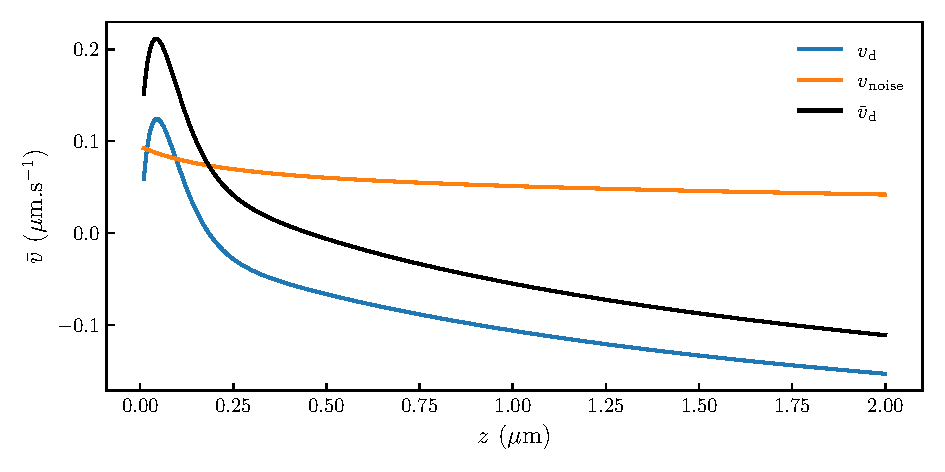
\includegraphics{02_body/chapter3/images/spurious_drift/spurious.pdf}
	\caption{Theoretical drift velocity for a colloidal particle of radius $a = 1.5 ~\mathrm{\mu m}$ in water and at a distance $z$ from the wall. The physical parameters $\ell_\mathrm{D} = 50 ~ \mathrm{nm}$, $B = 4 $ and $\ell_\mathrm{B} = 500 ~ \mathrm{nm}$. \href{https://github.com/eXpensia/Confined-Brownian-Motion/blob/main/02_body/chapter3/images/spurious_drift/spurious_drift.ipynb}{\faGithub}} 
	\label{fig.spurious}
\end{figure}


\subsubsection{Numerical simulations of confined Brownian motion}

We previously determined that the simulation of a bulk Brownian motion without external forces can be simulated using Eq.~(\ref{Eq.shortnumlangevin}).
However, in the case of confined Brownian motion, and without density matching, one needs to take into account the hindered mobility, external forces due to gravity and the double-layer interaction, as well as the confinement-induced spurious drift. Putting all that together leads to a new equation for $x_i$ which reads for the motion parallel to wall (\textit{i.e.} along the $x$- and $y$-axes):

\begin{equation}
	x_i = x_{i-1} +  \sqrt{2D_\parallel}w_i ~,
	\label{eq.langevinnearx}
\end{equation}

where we recall that we approximate the continuous position $X_t$ of a particle at a time $t$ by a discrete-time sequence $x_i$, which is the solution of the equation at a time $t_i = i\tau$. $\tau$ being the numerical integration time increment, and $w_i$ is a Faussian-ditributed number of mean value $\langle w_i \rangle =0$ and variance $\langle w_i ^2\rangle = \tau$. For the particle perpendicular motion (along the $z$-axis), one needs to add the total drift $\bar{v}_\textnormal{d}$ of Eq.~(\ref{Eq.total_drifts}), such that:

\begin{equation}
	z_i = z_{i-1} + \bar{v}_\mathrm{d}(z_{i-1}) \tau + \sqrt{2D_\bot}w_i ~,
	\label{eq.langevinnearz}
\end{equation}

 where $z_i$ is the discrete-time position sequence of a particle along the $z$-axis. Compared to bulk Brownian motion where the time step $\tau$ can be chosen only according to the desired precision as shown previously on Fig.~\ref{fig:MSEwi}, confinement adds another constraint. Indeed, the time step should be short enough for the drift $\bar{v}_\textnormal{d}$ and local diffusion coefficients to be relatively constant (as detailed later) in the time period $t_{i+1} - t_i = \tau$ and in the displacement range $\Delta z = z_{i+1} - z_i$, such that:

\begin{equation}
	\bar{v}_\mathrm{d} (z \in [z_i, z_{i+1}]) \simeq \bar{v}_\mathrm{d} (z_i) ~,
	\label{driftc}
\end{equation}

and:

\begin{equation}
	D_{\bot, \parallel}(z \in [z_i, z_{i+1}]) \simeq D_{\bot, \parallel}(z_i) ~.
\end{equation}

Since the diffusion coefficient does not vary for the parallel motion, one can consider only the perpendicular motion to determine the optimal simulation time step. Also, as it can be seen in Fig.~\ref{fig.taumax} the relative variation of the drift velocity $1/\bar{v}_\mathrm{d} \partial_z \bar{v}_\mathrm{d}$ reaches higher values than the relative variation of the diffusion coefficient $1/D_\bot \partial_z D_\bot$. Thus, finding $\tau$ that satisfies Eq.~(\ref{driftc}) is sufficient. Moreover, the vertical drift velocity varies more when the colloid is near the surface, \textit{i.e.} in the region where one can approximate the diffusion coefficient $D_\bot$ using Eqs.~(\ref{Eq.hindered})~and~(\ref{Eq:etaz_small}):

\begin{equation}
	\left.D_\bot  (z)\right|_{z\ll a} = D_ 0 \frac{z}{a} ~.
	\label{Dsmall}
\end{equation}

In that case, Eq.~(\ref{Eq.total_drifts}) near the surface simplifies to:

\begin{equation}
	\begin{aligned}
		\bar{v}_\textnormal{d} &\simeq  \frac{k_\mathrm{B}T}{\gamma_0} \frac{z}{a} \left[\frac{B}{\ell_\mathrm{D}} \exp \left(-\frac{z}{\ell_\mathrm{D}}\right) - \frac{1}{\ell_{\mathrm{B}}}  \right] + \frac{\partial}{\partial z} D_0 \frac{z}{a} \\
		&= \frac{D_0}{a} \left[ 1 + \frac{Bz}{\ell_\mathrm{D}} \exp \left(-\frac{z}{\ell_\mathrm{D}}\right)- \frac{1}{\ell_{\mathrm{B}}}\right]
	\end{aligned}
\end{equation}

By expanding the exponential term at the first order in $z/\ell_\mathrm{D}$, we get:

\begin{equation}
	\begin{aligned}
		\bar{v}_\textnormal{d}  = \frac{D_0}{a} \left( 1 + \frac{B z}{\ell_\mathrm{D}} - \frac{1}{\ell_{\mathrm{B}}}\right)
	\end{aligned}
	\label{drifts_short}
\end{equation}

To satisfy Eq.~(\ref{driftc}), we need to have a small relative change of the vertical drift velocity in an interval $[z, z+\Delta z]$ \cite{matse_state-dependent_nodate}, \textit{i.e.}:

\begin{equation}
	\frac{|\bar{v}_\mathrm{d} (z + \Delta z) - \bar{v}_\mathrm{d} (z)|}{|\bar{v}_\mathrm{d} (z)|} \ll 1 ~.
	\label{condition_drift}
\end{equation}

Combining Eqs.~(\ref{drifts_short})~and~(\ref{condition_drift}), we get:

\begin{equation}
	|\Delta z |\ll \left[\frac{B}{\ell_{\mathrm{D}}}\right]^{-1} + z ~.
	\label{inegality}
\end{equation}


Besides, invoking the vertical \gls{MSD} over the time step, as well as Eq.~(\ref{Dsmall}), one gets:

\begin{equation}
	\langle \Delta z ^2 \rangle (z) = 2 D_\bot (z) \tau = 2D_0 \frac{z}{a}\tau ~.
	\label{msdshort}
\end{equation}

Combining Eqs.~(\ref{inegality})~and~(\ref{msdshort}) thus leads to:

\begin{equation}
	\tau = \frac{a\langle \Delta z ^2 \rangle }{2 D_0 z} \ll \frac{a}{2 D_0 } \frac{\left[\left(\frac{B}{\ell_\mathrm{D}} - \frac{1}{\ell_{\mathrm{B}}}\right)^{-1} + z\right] ^2}{z} = \tau_\mathrm{max} (z)~.
	\label{taumax}
\end{equation}

 At this point, there are two different options for the time step in the simulation: the first one is to do an adaptive time step using a local $\tau(z)$ that satisfies $\tau(z) \ll \tau_{\textrm{max}}(z)$ for each step of the simulation; the second one is to find the smallest $\tau_\mathrm{max}(z)$ and use for all the simulation a time step $\tau$ satisfying $\tau \ll \mathrm{min}(\tau_\mathrm{max}) $. The latter can be evaluated by finding the height $z_\mathrm{min}$, at which the derivative of $ \tau_\mathrm{max}$ nullifies, \textit{i.e.}:

\begin{equation}
	\left. \frac{\partial \tau_\mathrm{max}}{\partial z} \right| _{z_\mathrm{min} }= 0 ~.
\end{equation} 

Solving the latter gives,

\begin{equation}
	z_\mathrm{min} = \left| \left( \frac{B}{\ell_\mathrm{D}} - \frac{1}{\ell_{\mathrm{B}}}\right)^{-1} \right|~.
\end{equation}


which finally gives:

\begin{equation}
	\mathrm{min}(\tau_\mathrm{max}) =  \frac{2 a}{D_0}  \left| \left( \frac{B}{\ell_\mathrm{D}} - \frac{1}{\ell_{\mathrm{B}}}\right)^{-1} \right| ~.
\end{equation}

In Fig.~\ref{fig.taumax}-b) $\tau_{\mathrm{max}}$ is plotted as a function of $z$, for $a=1.5 ~\mathrm{\mu m}$, $B = 4$ and $\ell _\mathrm{D}$ varying between $20$ and $100$ nm. We observe that for this range of values that represents well the experiments that I have performed during my thesis, taking a constant simulation time step $\tau \approx 0.01 ~ \mathrm{s}$ is satisfactory.

\begin{figure}[H]
	\centering
	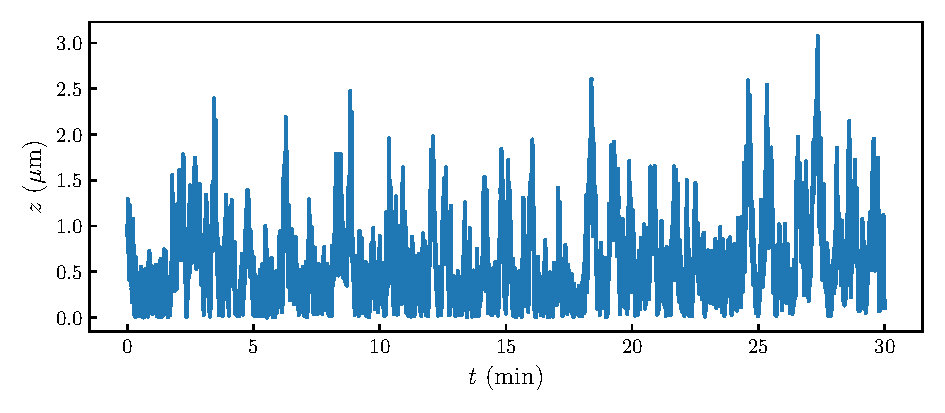
\includegraphics{02_body/chapter3/images/simulation_confined_Brownian_motion/z_traj_sim.pdf}
	\caption{Simulated trajectory along the direction normal to the wall, using Eq.~(\ref{eq.langevinnearz}) with $\alpha = 1$ (isothermal convention), of radius $a= 1.5  ~ \mathrm{\mu m}$, density $\rho_\mathrm{p} = 1050  ~\mathrm{kg.m^{-3}}$, placed in water near a wall. The particle-wall interaction is characterized by $\ell_\mathrm{D} = 50$ nm and $B=4$. \href{https://github.com/eXpensia/Confined-Brownian-Motion/blob/main/02_body/chapter3/images/simulation_confined_Brownian_motion/Overdamped_confined_simulation.ipynb}{\faGithub}} 
	\label{fig.z_traj_confined_simulated}
\end{figure}

\begin{figure}[H]
	\centering
	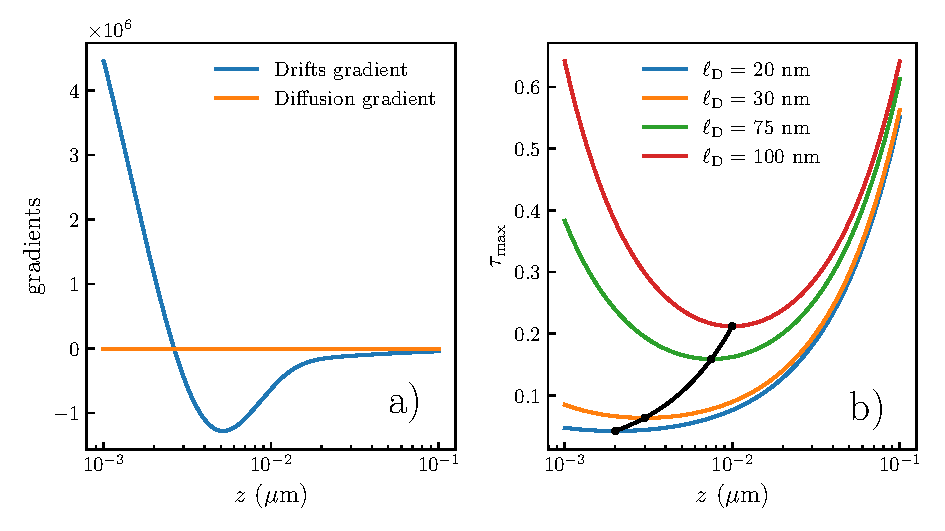
\includegraphics{02_body/chapter3/images/simulation_confined_Brownian_motion/maximal_tau.pdf}
	\caption{a) Theoretical computation of the relative variation of the drift velocity $\bar{v}_\mathrm{d}$ and perpendicular diffusion coefficient $D_\bot$ as a function particle-wall distance $z$. The parameters are $\ell_\mathrm{D}=50$, $B=4$ and $\ell_{\mathrm{B}} = 500$ nm b) Optimal numerical integration time step $\tau_\mathrm{max}$ as a function of the particle-wall distance $z$ for a particle of radius $a = 1.5 ~\mathrm{\mu m}$, with $\ell_{\textrm{B}}=500$~nm, $B = 4$, and for different Debye lengths as indicated. The black line connects the minima.\href{https://github.com/eXpensia/Confined-Brownian-Motion/blob/main/02_body/chapter3/images/simulation_confined_Brownian_motion/maximal_tau.ipynb}{\faGithub}} 
	\label{fig.taumax}
\end{figure}


We have developed the numerical simulation of Eqs.~(\ref{eq.langevinnearx})~and~(\ref{eq.langevinnearz}) using Python, as part of the Master's internship of Élodie Millan. The interested reader will find more information on  the simulation of confined Brownian motion in complex systems in her forthcoming thesis. A typical trajectory of a water-immersed colloidal particle of radius $a= 1.5  ~ \mathrm{\mu m}$ and density $\rho_\mathrm{p} = 1050  ~\mathrm{kg.m^{-3}}$, near a wall with which the electrostatic interaction is characterized by $\ell_\mathrm{D} = 50$ nm and $B=4$, is plotted in Fig.~\ref{fig.z_traj_confined_simulated}.It qualitatively resembles experimental trajectory that was shown in Fig.~\ref{Fig:exp_z_traj} as an introduction to the chapter. In this trajectory, the noise-induced lift is taken into account by using the isothermal convention (\textit{i.e.} $\alpha =1 $). To check if the spurious drift is correctly implemented, the constraint we have is that the long-time statistics should satisfy Eq.~(\ref{Eq.Peq}). To compute an experimental probability density function from a set of points, one can use the following Python snippet.

\newpage
\begin{minted}
	[
	frame=lines,
	framesep=2mm,
	baselinestretch=1.2,
	fontsize=\footnotesize,
	linenos
	]
	{python}
def pdf(data, bins=10, density=True):
	
  pdf, bins_edge = np.histogram(data, bins=bins, density=density)
  bins_center = (bins_edge[0:-1] + bins_edge[1:]) / 2
	
  return pdf, bins_center
\end{minted}

The long-time \gls{PDF} in position, for with and without the spurious drift $v_\mathrm{spurious}$ are shown in Fig.~\ref{fig.pdf_vs_alpha}. We see that the spurious drift velocity $v_\mathrm{spurious}$ permits retrieving the correct distribution. In the case ($v_\mathrm{spurious} = 0$), we observe that the particle is more likely to be found closer to the surface, as a result of the missing compensating spurious drift of Eq.~(\ref{Eq.spurious_drift}).

\begin{figure}[H]
	\centering
	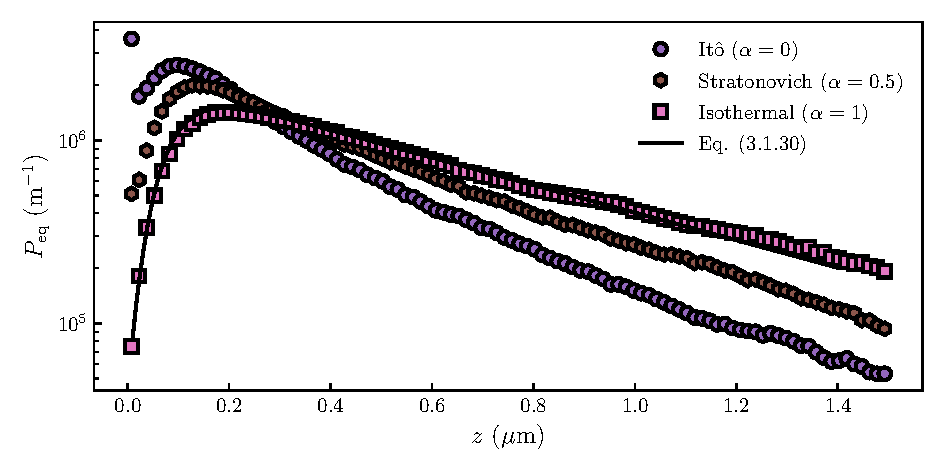
\includegraphics{02_body/chapter3/images/simulation_confined_Brownian_motion/Peq_vs_alpha.pdf}
	\caption{Simulated, Long-term Probability Density Function of the height of the particle with or without the spurious drift, as indicated. The solid black line represents the expected Gibbs-Boltzmann distribution. The physical parameters are: $a = 1.5 ~ \mathrm{\mu m}$, $\rho_\mathrm{p} = 1050 ~\mathrm{kg.m^{-3}}$, $\ell_\mathrm{D} = 50$ nm, $B = 4$ and $\ell_\mathrm{B} = 577$ nm. \href{https://github.com/eXpensia/Confined-Brownian-Motion/blob/main/02_body/chapter3/images/simulation_confined_Brownian_motion/Overdamped_confined_simulation.ipynb}{\faGithub}}
	\label{fig.pdf_vs_alpha}
\end{figure}


\subsection{Experimental study}
\label{section:expresults}
Let us now analyze the experimental data acquired through the Mie tracking (see section \ref{chap:LM_fit}). In the near-wall Brownian dynamic theory presented section~\ref{sec:confined}, we considered distance $z$ between the wall and the colloidal particle surface. However, it is not the height measured by the Mie tracking, since the latter measures the distance between the objective-lens focal plane and the particle center. Therefore, we measure the trajectory up to an offset, \textit{i.e.} the objective-lens focal plane to wall distance. To have the correct measured height, we suppose that the particle does approach very closely to the wall, such that the minimal measured distance is the focal plane to the wall distance. From that assumption, we set the minimal value of $z$ in the trajectory to zero. This is repeated periodically and thus termed the moving-minimum method, and can be calculated using the following Python function.



\begin{minted}
	[
	frame=lines,
	framesep=2mm,
	baselinestretch=1.2,
	fontsize=\footnotesize,
	obeytabs=true,
	tabsize=2,
	linenos
	]
	{python}
def movmin(z, window):
	result = np.empty_like(z)
	start_pt = 0
	end_pt = int(np.ceil(window / 2))
	
	for i in range(len(z)):
		if i < int(np.ceil(window / 2)):
			start_pt = 0
		if i > len(z) - int(np.ceil(window / 2)):
			end_pt = len(z)
			
		result[i] = np.min(z[start_pt:end_pt])
		start_pt += 1
		end_pt += 1
	return result
\end{minted}

In the above snippet, \mintinline{python}{window} represents the number of points used to compute the minimum. As an example, if one chooses \mintinline{python}{window = 100}, the first value of \mintinline{python}{result} is the minimum of the first 100 points of \mintinline{python}{z}. If there is enough data around the point where the minimum is calculated, the ensemble is centered, with a new window of size 100 (\textit{i.e.} \mintinline{python}|result[100] = np.min(z[50:150])|. If there is not enough point around the $n$-th point, we then take the average value of the first (or the last) $n$ points. The raw and shifted trajectories are shown  in Fig.~\ref{fig.rescaled_traj}. Moreover, subtracting the moving minimum has a benefit. Indeed, it can remove some experimental drift due to the mechanical movement of the optical pieces of the microscope. Also, due to the approximation made to use the moving-minimum method, the exact location of the $z=0$ origin is \textit{a priori} undetermined we need to add to the physical parameters $B$, $\ell_\mathrm{D}$ and $\ell_\mathrm{B}$ a forth parameter: the height offset $z_\mathrm{off}$ that accounts for the correction of the wall position.

\begin{figure}[ht]
	\centering
	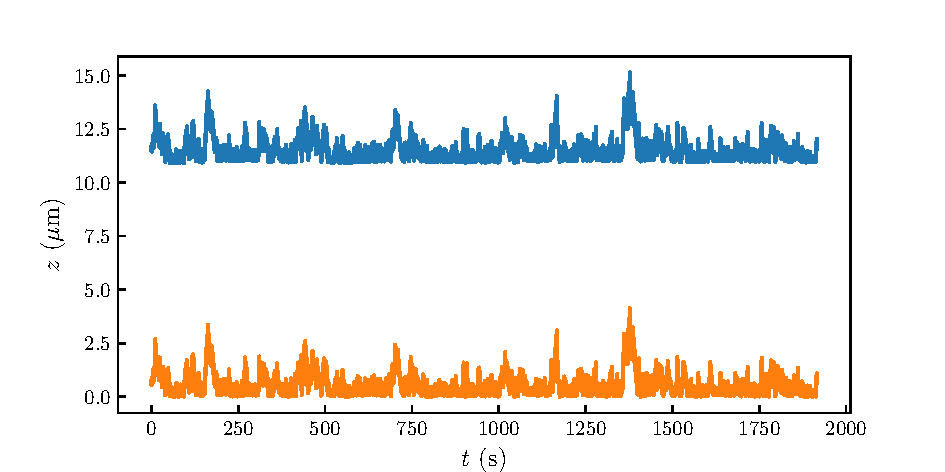
\includegraphics{02_body/chapter3/images/trajctory_analysis/traj_rescaled.pdf}
	\caption{Raw trajectories measured using the Mie-tracking technique, and it shifted version (bottom, orange) using the moving-minimum method with a window of $10000$ points.~\href{https://github.com/eXpensia/Confined-Brownian-Motion/blob/main/02_body/chapter3/images/trajctory_analysis/graph_ploting.ipynb}{\faGithub}} 
	\label{fig.rescaled_traj}
\end{figure}

\subsubsection{Equilibrium distribution}
\label{sec:Eqdistrib}

As we have done for the simulated trajectory, one can construct the equilibrium probability density function $P_\mathrm{eq}(z)$ of the position of the particle. As seen in Fig.~\ref{fig.pdf_exp}, and explained in section \ref{sec:gravit}, an exponential tail is observed at large distance, which is identified to the sedimentation contribution in Perrin's experiment~\cite{perrin_les_2014}, but here with the probability density function of a single particle instead of the concentration field. In contrast, near the wall, we observe an abrupt depletion, indicating a repulsive electrostatic contribution. Additionally, we see that the Gibbs-Boltzmann distribution of Eq.~(\ref{Eq.Peq}) fits the data very well.



Moreover, as shown in Fig.~\ref{fig.ld}, we recover the Debye relation, \textit{i.e.} $\ell_{\mathrm{D}}=0.304/\sqrt{\textrm{[NaCl]}}$ (see Eq.~(\ref{ldnacl})), with $\ell_{\mathrm{D}}$ in nm, and where [NaCl] is the concentration of salt in mol/L , with a prefactor corresponding to a single monovalent salt in water at room temperature~\cite{israelachvili_intermolecular_2015}. Besides, we have verified, as shown in Fig.~\ref{fig.ld}, that the dimensionless parameter $B$ related to surface charges is constant in the studied salt-concentration range, thus excluding any nonlinear effect~\cite{wang_measurement_2011,oberholzer_grand_1997} in our case. 

\begin{figure}[h!]
	\centering
	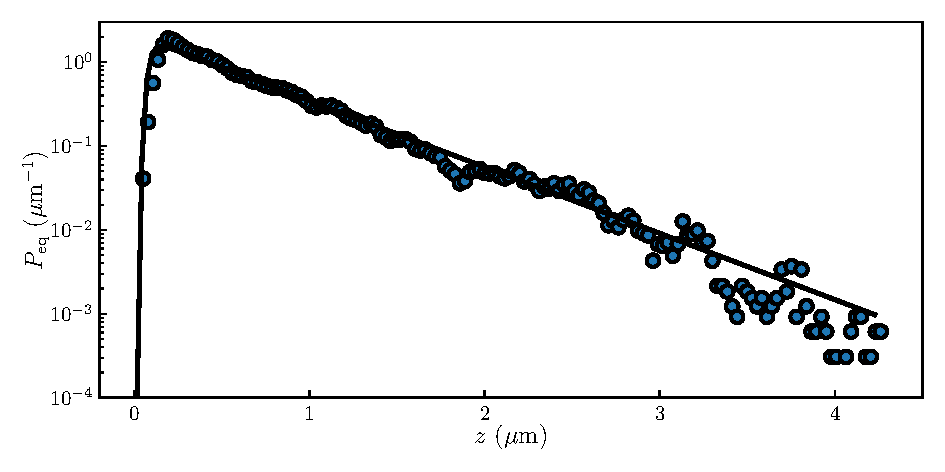
\includegraphics{02_body/chapter3/images/trajctory_analysis/pdf_exp.pdf}
	\caption{Measured equilibrium probability density function $P_{\textrm{eq}}$ of the distance $z$ between the particle and the wall. The solid line represents the best fit to the normalized Gibbs-Boltzmann distribution in position, using the total potential energy $U(z)$ of Eq.~(\ref{Eq:PDF}), with $B = 4.8$, $\ell_\mathrm{D} = 21 ~ \mathrm{nm}$, and $\ell_\mathrm{B} = 530~ \mathrm{nm}$.~\href{https://github.com/eXpensia/Confined-Brownian-Motion/blob/main/02_body/chapter3/images/trajctory_analysis/graph_ploting.ipynb}{\faGithub}}
	\label{fig.pdf_exp}
\end{figure}


\begin{figure}[H]
	\centering
	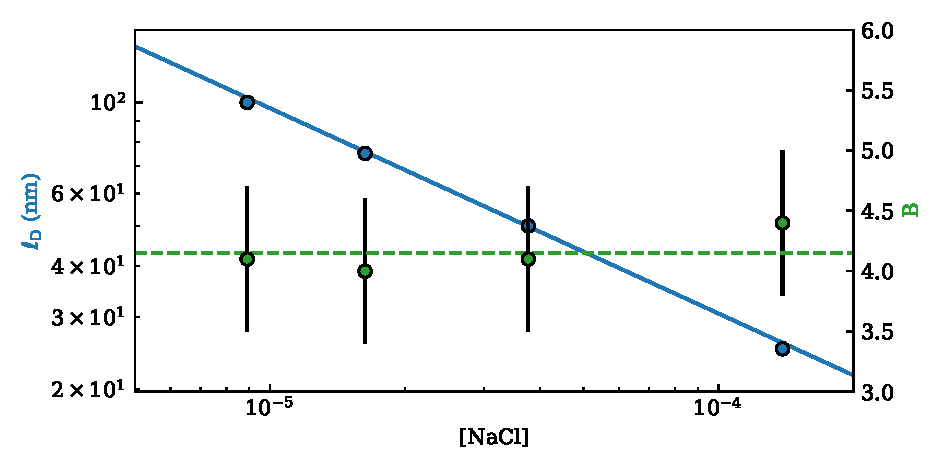
\includegraphics{02_body/chapter3/images/trajctory_analysis/ld.pdf}
	\caption{In blue, left axis, measured Debye length $\ell_\mathrm{D}$ as a function of salt concentration [NaCl]. The solid line is the expected Debye relation $\ell_\mathrm{D}=0.304/\sqrt{\textrm{[NaCl]}}$, for a single monovalent salt in water at room temperature. In green, right axis, measured $B$ as a function of salt  concentration [NaCl]. The dashed line represents the mean value of the measured $B$ values.~\href{https://github.com/eXpensia/Confined-Brownian-Motion/blob/main/02_body/chapter3/images/trajctory_analysis/resume_ld_measures.ipynb}{\faGithub}}
	\label{fig.ld}
\end{figure}


\subsubsection{Mean Square Displacement}

We now turn to dynamical aspects, by considering the mean-squared displacement (MSD). We recall that, for the three spatial directions, indexed by $i=x$, $y$, and $z$, corresponding to the coordinates $r_x=x$, $r_y=y$, and $r_z=z$, of the position $\vec{r}$, and for a given time increment $\Delta t$, the MSD is defined as:
\begin{equation}
	\langle\Delta r_i(t)^2 \rangle_t = \langle[r_i(t+\Delta t) - r_i(t)]^2\rangle_t\ ,
	\label{MSDdef}
\end{equation}
where the average $\langle\rangle_t$ is performed over time $t$. For a free Brownian motion in the bulk, and in the absence of other forces than the dissipative and random ones, the \gls{MSD} is linear in time, \textit{i.e.} $\langle\Delta r_i(t)^2 \rangle_t = 2 D_0 \Delta t$, where is the bulk diffusion coefficient (see Eq.~(\ref{Eq.D})) given by the Stokes-Einstein relation~\cite{einstein_uber_1905}. Further including sedimentation restricts the validity of the linearity of the \gls{MSD} along the $z$-axis to short times only, \textit{i.e.} for $\Delta t\ll\ell_{\textrm{B}}^2/D_0$ such that the vertical diffusion is not yet affected by the gravitational drift.

As explain in section \ref{subsec:double} The presence of a rigid wall at $z=0$ adds a repulsive electrostatic force along $z$. It also decreases the mobilities nearby through hydrodynamic interactions (see section \ref{sec:diff}), where we recall that it leads to effective viscosities $\eta_\parallel(z)=\eta_x(z)=\eta_y(z)$, and $\eta_\bot(z) = \eta_z(z)$ (see Eq.\ref{Eq.hindered}). Interestingly, despite the previous modifications, the temporal linearity of the MSD is not altered by the presence of the wall~\cite{chubynsky_diffusing_2014,prieve_measurement_1999} for $x$ and $y$, as well as at short times for $z$. In such cases, the MSD reads:
\begin{equation}
	\langle\Delta r_i(t)^2 \rangle_t = 2 \langle D_i \rangle \Delta t\ ,
	\label{averagediff}
\end{equation}

where we introduced and the average of the local diffusion coefficient:

\begin{equation}
	\langle D_i(z) \rangle = \int_0^{\infty} \textrm{d}z\, D_i(z)P_{\textrm{eq}}(z) ~,
\end{equation}  

against the Gibbs-Boltzmann distribution in position. As shown in Fig.~\ref{fig.MSD}, the MSD measured along $x$ or $y$ is indeed linear in time. By fitting the data to Eq.~(\ref{averagediff}), using Eqs.~(\ref{Eq:PDF})~and~(\ref{Eq:etax}), we extract an average transverse diffusion coefficient $\langle D_\parallel \rangle= \langle D_x\rangle=\langle D_y \rangle= 0.52\, D_0$. In contrast, along $z$, we identify two different regimes: one at short times, where the \gls{MSD} is still linear in time, with a similarly-obtained best-fit value of $\langle D_z \rangle= 0.24\, D_0$; and one at long times, where the MSD saturates to a plateau. This latter behavior indicates that the equilibrium regime has been reached, with the particle having essentially explored all the relevant positions given by the Gibbs-Boltzmann distribution.

\begin{figure}[t!]
	\centering
	\includegraphics{02_body/chapter3/images/trajctory_analysis/msd.pdf}
	\caption{Measured mean-squared displacements (MSD, see Eq.~(\ref{MSDdef})) as functions of the time increment $\Delta t$, for the three spatial directions, $x$, $y$, and $z$. The solid lines are best fits to Eq.~(\ref{averagediff}), using Eqs.~(\ref{Eq:PDF}),~(\ref{Eq:etaz})~and~(\ref{Eq:etax}), with $B = 4.8$, $\ell_\mathrm{D} = 21 ~ \mathrm{nm}$, and $\ell_\mathrm{B} = 530~\mathrm{nm}$,
		providing the average diffusion coefficients $\langle{D_\parallel}\rangle= \langle D_x\rangle=\langle D_y \rangle =0.52\,D_0$ and $\langle D_z \rangle =0.24\, D_0$. The dashed line is the best fit to Eq.~(\ref{Eq:plateau}), using Eq.~(\ref{Eq:PDF}), with $B = 4.8$, $\ell_\mathrm{D} = 21 ~ \mathrm{nm}$, and $\ell_\mathrm{B} = 530~\mathrm{nm}$.~\href{https://github.com/eXpensia/Confined-Brownian-Motion/blob/main/02_body/chapter3/images/trajctory_analysis/graph_ploting.ipynb}{\faGithub}}
	\label{fig.MSD}
\end{figure}


\subsubsection{Non-Gaussian dynamics - displacement distribution}

Having focused on the \gls{MSD}, \textit{i.e.} on the second moment only, we now turn to the full-Probability Density Function $P_i$ of the displacement $\Delta r_i$. Since the diffusion coefficient $D_i(z)$ varies as a result of the variation of $z$ along the particle trajectory, $P_i$ exhibits a non-Gaussian behavior, as seen in Figs.~\ref{fig.displacement}-a,b,c,d). We even resolve the onset of a non-Gaussian behavior in $P_x$, by zooming on the large-$\lvert\Delta x\rvert$ wings. At short times, the diffusion coefficient $D_i$ and the drift velocity $\bar{v}_\mathrm{d}$, can be considered constant. By writing the initial condition of the particle-wall distance $\delta(z - z_0)$, the solution of Eq.~(\ref{final_fokker}) becomes:

\begin{equation}
	\begin{aligned}
		P_z(z, z_0, \Delta t) &= \exp \left[  \frac{\partial ^2}{\partial z ^2} D_\bot(z_0) \Delta t - \frac{\partial}{\partial z} \bar{v} _\mathrm{d} (z_0) \Delta t \right] \frac{1}{2 \pi} \int _{-\infty} ^{\infty} ~ \textnormal{d}u \exp (ju(z-z_0))  \\
		& = \frac{1}{2\pi} \int_{-\infty}^{\infty} ~ \textnormal{d}u \exp \left[ -u^2 D_\bot(z_0)\Delta t + ju(z-z_0) - ju  \bar{v} _\mathrm{d} (z_0) \Delta t \right] ~.
	\end{aligned}
\end{equation}

The latter can be reduced to \cite{matse_state-dependent_nodate, risken_fokker-planck_2012}:

\begin{equation}
	P_z(\Delta z, z_0, \Delta t) =   \frac{1}{\sqrt{4 \pi D_i(z_0) \Delta t}} \exp \left[-\frac{(\Delta r_i - \bar{v}_\mathrm{d}\Delta t)^2}{4 D_i(z_0) \Delta t}   \right]\ ,
	\label{Pdxshort}
\end{equation}
which is a Gaussian distribution with a mean value $\langle \Delta z \rangle =  \bar{v}_\mathrm{d}\Delta t$. The same calculus can be done for the $x$- and $y$-axes, by setting the drift velocity to zero and using $D_\bot$. Additionally, it has a standard deviation $\sigma_i(z_0) = \sqrt{2D_i (z_0) \Delta t}$. From Eq.~(\ref{Pdxshort}), we can observe than the total drift $\bar{v}_\mathrm{d}$ induces an asymmetry on the displacement along the $z$-axis. However, in our experiment, as we have access to long-enough trajectories to reach equilibrium, we are conditioned by the initial position but by the Gibbs-Boltzmann distribution of Eq.~(\ref{Eq.Peq}). At short times, $P_i$ can thus be modeled by the averaged diffusion Green's function~\cite{matse_test_2017,hapca_anomalous_2009}:
\begin{equation}
	\begin{aligned}
		P_i(\Delta r_i, \Delta t) & = \int _{0} ^\infty ~\textnormal{d} z P_\mathrm{eq} (z) P(\Delta r_i, z, \Delta t) \\
		&= \int ^\infty _0 \mathrm{d}z\, P_{\textrm{eq}}(z) \frac{1}{\sqrt{4 \pi D_i(z) \Delta t}} \textrm{e}^{-\frac{\Delta r_i^2}{4 D_i(z) \Delta t}     }\ ,
	\end{aligned}
	\label{Eq:PDzshort}
\end{equation}
against the Gibbs-Boltzmann distribution. The latter equation can alternatively be written as an integral over the diffusion coefficient such that:
\begin{equation}
	P_i(\Delta r_i , \Delta t) = \int_0 ^\infty \mathrm{d}D_iP(D_i) \frac{1}{\sqrt{4 \pi D_i \Delta t}} \mathrm{e} ^{\frac{-\Delta r_i ^2}{4D_i\Delta t}} 
\end{equation}

This equation can be evaluated using the following Python snippet.

\begin{minted}
	[
	frame=lines,
	framesep=2mm,
	baselinestretch=1.2,
	fontsize=\footnotesize,
	linenos
	]
	{python}
def P_D(B, ld, lb):
  # Computing the D PDF.
  z = np.linspace(1e-9, 15e-6, 1000)
  P_D = Dz(z) * P_b_off(z, offset, B, ld, lb)
  P_D = P_D / np.trapz(P_D, z)  # extra step to ensure PDF normalization
  return Dz, P_D
	
	
def _P_Dz_short_time(Dz, Dt, B, ld, lb):
  # Using the D PDF to compute P()
  D_z, P_D = P_D(B, ld, lb)
  P = P_D / np.sqrt(4 * np.pi * D_z * Dt) * np.exp(-(Dz ** 2) / (4 * D_z * Dt))
  P = np.trapz(P, D_z)
  return P
	
	
	# Creating a handy function for easier use with Dz numpy arrays
def P_Dz_short_time(Dz, Dt, B, ld, lb):
  P = np.array([_P_Dz_short_time(i, Dt, B, ld, lb) for i in Dz])
  P = P / np.trapz(P, Dz) # extra step to ensure PDF normalization
  return P
\end{minted}

In this snippet, the evaluation is done for $\Delta z$. However, when computing $P_x(\Delta x)$ one should just change the \mintinline{python}{Dz(z)} function to $D_\parallel$. Since $P$ is a \gls{PDF}, it should be normalized such that $\int P = 1$. We added an extra step to ensure \gls{PDF} normalization along the evaluation.
At long time enough, since we have reached equilibrium, the averaged particle's drift should be equal to zero thus leading to a mean value $\langle \Delta r_i \rangle_t  = 0$. As shown in Figs.\ref{fig.displacement}-a,c,b,d) Eq.~(\ref{Eq:PDzshort}) captures the early data very well. At long times, Eq.~(\ref{Eq:PDzshort}) remains valid only for $P_x$ and $P_y$. Nevertheless, the equilibrium regime being reached, $P_z$ only depends on the Gibbs-Boltzmann distribution. Indeed, in this regime $P_z$ can be written as a convolution of two Gibbs-Boltzmann distribution as in a displacement $\Delta z = z(t+\Delta t) - z(t)$, $ z(t+\Delta t)$ and  $z(t)$ comes from independent draw from the Gibbs-Boltzmann distribution:
\begin{equation}
	\lim_{\Delta t\rightarrow\infty}P_z(\Delta z, \Delta t) = \int_0^{\infty}\textrm{d}z\,P_{\textrm{eq}}(z+\Delta z)P_{\textrm{eq}}(z)\ ,
	\label{auxiliary}
\end{equation}
which contains in particular the second moment:
\begin{equation}
	\lim_{\Delta t\rightarrow\infty}\langle\Delta z ^2\rangle = \int _{- \infty} ^{+ \infty}\textrm{d}\Delta z\, \Delta z^2\int_0^{\infty}\textrm{d}z\, P_{\textrm{eq}}(z+\Delta z)P_{\textrm{eq}}(z) \ .   
	\label{Eq:plateau}
\end{equation}

As shown in Fig.~\ref{fig.displacement}-e), Eq.~(\ref{auxiliary}) captures the long-term data along $z$ very well. Additionally, Eq.~(\ref{Eq:plateau}) permits to fit the long-term plateau of the \gls{MSD} shown in Fig.~\ref{fig.MSD}. Eq.~(\ref{auxiliary}) can be evaluated using the following Python function:


\begin{minted}
	[
	frame=lines,
	framesep=2mm,
	baselinestretch=1.2,
	fontsize=\footnotesize,
	linenos
	]
	{python}
def _Pdeltaz_long(DZ, B, ld, lb):
  z = np.linspace(0, 20e-6, 1000)    
  dP = P_eq(z, B, ld, lb) * P_eq(z + DZ, B, ld, lb)
  P = trapz(dP,z)
  return P
	
def Pdeltaz_long(DZ, B, ld, lb):
  pdf = np.array([_Pdeltaz_long(i,B, ld, lb) for i in DZ])
  pdf = pdf / trapz(pdf,DZ)
  return pdf
	
\end{minted}

where the \mintinline{python}{P_eq} function has been described in section \ref{Section:sphere-wall}. 


\begin{figure}[H]
	\centering
	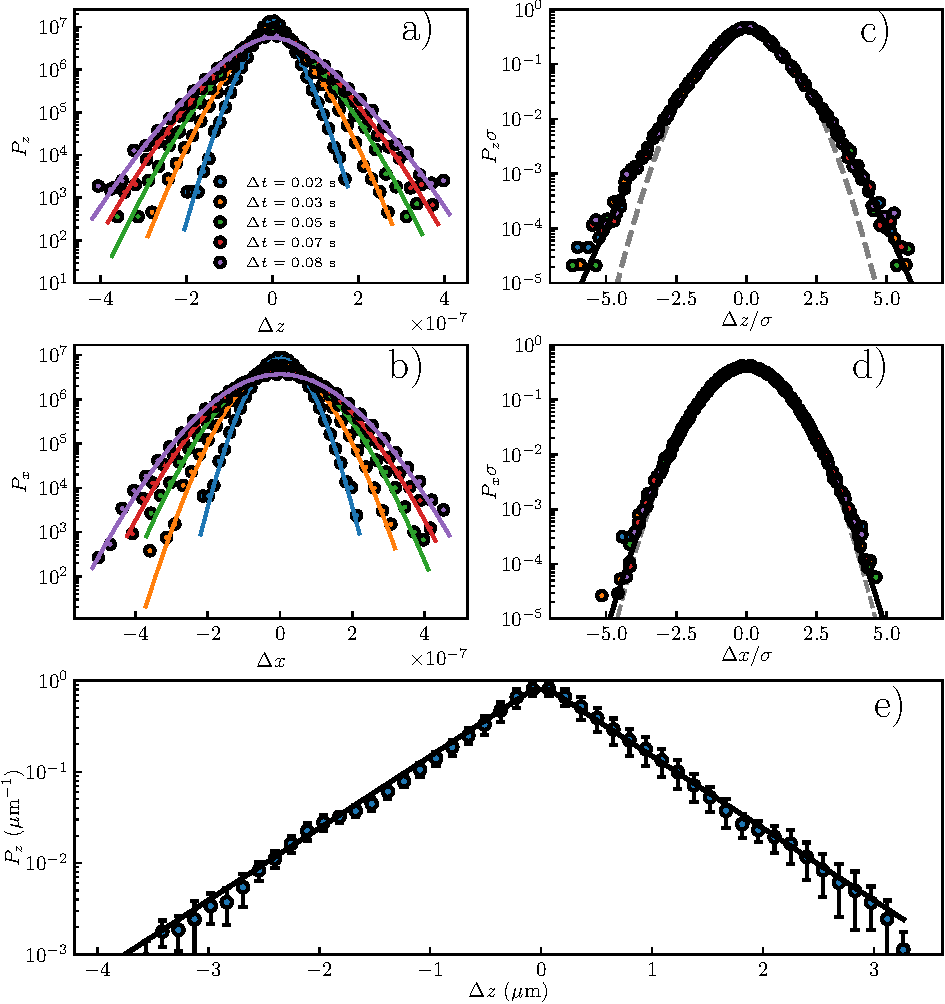
\includegraphics{02_body/chapter3/images/trajctory_analysis/P_displacement.pdf}
	\caption{a, b) Probability density functions $P_i$ of the displacements $\Delta x$ and $\Delta z$, at short times. The solid lines are the best fits to Eq.~(\ref{Eq:PDzshort}), using Eqs.~(\ref{Eq.Peq}),~(\ref{Eq:etaz}),~and~(\ref{Eq:etax}), with $B = 4.8$, $\ell_\mathrm{D} = 21 ~ \mathrm{nm}$, and $\ell_\mathrm{B} = 530~\mathrm{nm}$. c,d) Normalized probability density functions $P_i\,\sigma$ of the normalized displacements $\Delta x/\sigma$ and $\Delta z/\sigma$, at short times, with $\sigma^2$ the corresponding MSD (see Fig.~\ref{fig.MSD}), for different time increments $\Delta t$ ranging from 0.0167~s to 0.083~s, as indicated with different colors. The solid lines are the best fits to Eq.~(\ref{Eq:PDzshort}), using Eqs.~(\ref{Eq:PDF}),~(\ref{Eq:etaz}),~and~(\ref{Eq:etax}), with $B = 4.8$, $\ell_\mathrm{D} = 21 ~ \mathrm{nm}$, and $\ell_\mathrm{B} = 530~\mathrm{nm}$. For comparison, the gray dashed lines are normalized Gaussian distributions, with zero means and unit variances. d) Probability density function $P_z$ of the displacement $\Delta z$, at long times, averaged over several values of $\Delta t$ ranging between 25 s and 30~s. The solid line is the best fit to Eq.~(\ref{auxiliary}), using Eq.~(\ref{Eq:PDF}), with $B = 4.8$, $\ell_\mathrm{D} = 21 ~ \mathrm{nm}$, and $\ell_\mathrm{B} = 530~\mathrm{nm}$.}
	\label{fig.displacement}
\end{figure}



\subsubsection{Local diffusion coefficient}

We now wish to go beyond the previous average $\langle D_i\rangle$ of Eq.~(\ref{averagediff}), and resolve the local diffusion coefficient $D_i(z)$. To measure local viscosities from experimental trajectories, a binning method is generally employed~\cite{friedrich_approaching_2011}. This method computes the average $\langle ( \Delta r_i^2 ) (z)$ locally over a $z$-binning grid such that the local diffusion coefficient writes:

\begin{equation}
	D_i(z) = \frac{\langle  \Delta r_i^2  \rangle _t (z)}{\Delta t} ~.
	\label{binning}
\end{equation}

Using this method, Vestergard \textit{et al.} \cite{vestergaard_estimation_2015} discovered that the obturation time of the camera and the localization error $\sigma_{\mathrm{r}_i}$ plays an important role in the determination of the local diffusion coefficient such that Eq.~\ref{binning} should be rewritten as:

\begin{equation}
	D_i(z) = \frac{\langle  \Delta r_i^2 \rangle _t (z) - 2 \sigma_{\mathrm{r}_i}^2}{2(1 - R)\Delta t}~.
	\label{binning_vestergaard}
\end{equation}

where $R$ is a motion blur coefficient that depends on the aperture time of the camera. Let us write $\tau$ the time lapse between the capture of two images, and $\zeta(t)$ the state of the camera shutter during this time-lapse. $\zeta(t) > 0$ indicates that an open shutter while  $\zeta(t) = 0$ indicates a close shutter. The scale $\zeta(t)$ is fixed by the normalization condition $\int_{0}^{\tau} \zeta(t)\textnormal{d}t$. The motion blur coefficient is given by:

\begin{equation}
	R = \frac{1}{\tau} \int_{0}^{\tau} S(t)[1 - S(t)] \textnormal{d}t,
\end{equation}

where $S(t) = \int_{0}^{t}\zeta(t') \textnormal{d}t'$. If the shutter is kept open for the whole duration of the time-lapse, one has $R = 1/6$. The localization error $\sigma_{\mathrm{r}_i}$ can be determined from a measured trajectory. Taking into account that Brownian motion should not be correlated, one can measure $\sigma_{\mathrm{r}_i}$ by calculated the autocorrelation $x_i(n)$ as a function of the number of time steps $n$ of the particle position $r_i$, which we defined as:

\begin{equation}
	x(n) =  \langle (r_i(t) - \langle r_i(t) \rangle_t  ) (r_i(t + n\Delta t) - \langle r_i(t) \rangle_t) \rangle_t ~.
\end{equation}

In \cite{vestergaard_estimation_2015} the localization error (also called Vestergaard error) is written as:

\begin{equation}
	\sigma_{\mathrm{r}_i} = \sqrt{x(1) - \frac{2 \langle \Delta r_i^2 \rangle_t }{1-R}}
\end{equation}
Moreover,  mechanical drifts (or evaporation driven-flow in the sample) can lead to correlation in the position time-series, such that $\sigma_{\mathrm{r}_i}$ increases in the presence of unwanted drifts. In our experience we had $\sigma_{\mathrm{r}_x} = \sigma_{\mathrm{r}_y} = 12$~nm and $\sigma_{\mathrm{r}_z} = 6$~nm. 



\begin{figure}[h!]
	\centering
	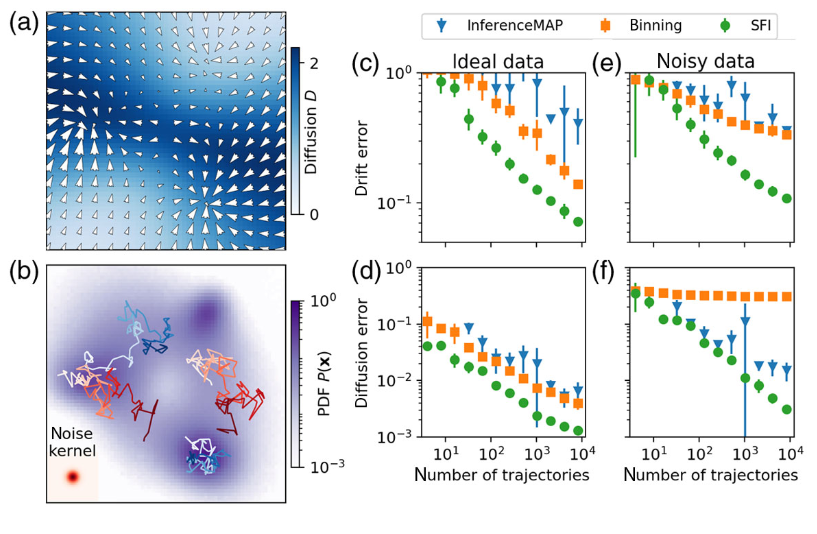
\includegraphics[scale=0.6]{02_body/chapter3/images/diffusion_coefficient/figure_Ronceray.png}
	\caption{Figure from \cite{frishman_learning_2020}. Quantitative comparison of Surface Force Inference (\gls{SFI} with other methods on a simulated system mimicking 2D single-molecule trajectories in a complex environment with space-dependent isotropic diffusion. a) The diffusion field (blue gradient) and drift field (white arrows). b) The steady-state distribution function (\gls{PDF}) of the process. The traces are representative trajectories of $100$ time steps. c-f) Comparison of the performance of \gls{SFI} and two widely used inference methods: InferenceMAP, a method for single-molecule inference (blue triangles)  \cite{beheiry_inferencemap_2015}, and grid-based binning with maximum-likelihood estimation \cite{hoze_heterogeneity_2012, friedrich_approaching_2011} (orange squares). They evaluated the performance of these methods on the approximation of the drift field (c),e)) and diffusion field (d)f)) as a function of the number $N$ of single-molecule trajectories (similar to the ones in panel b)) used. With ideal data (c),d)) and in the presence of measurement noise(e),f)). The performance is evaluated as the average mean-squared error on the reconstructed field along trajectories.  More information about the parameters of their simulation and analysis can be found in their work \cite{frishman_learning_2020}.}
	\label{fig.ronceray}
\end{figure}

Although the binning method is well suited for drift measurements, it suffers from a lack of convergence and precision when second moments or local diffusion coefficients have to be extracted. In particular, the binning method did not allow us to measure specifically the local diffusion coefficient in the key interfacial region corresponding to $z<100$~nm. Indeed, as we can observe in Fig.~\ref{fig.ronceray}-f) the diffusion error on noisy (such as experimental) data does saturate, and the binning method is outperformed by a robust method  recently developed by Frishman and Ronceray \cite{frishman_learning_2020}. This method uses Stochastic Force Inference (\gls{SFI}), in order to evaluate spatially varying force fields and diffusion coefficients, from the information contained within the trajectories. 

In practice the \gls{SFI} method computes a local diffusion estimator:

\begin{equation}
	\hat{d}(t_i) = \frac{[\Delta r_i (t_{i-1}) +\Delta r_i (t_{i}) ]^2}{4 \Delta t} + \frac{\Delta r_i (t_{i})\Delta r_i (t_{i-1})}{2\Delta t},
\end{equation}

where the second term corresponds to Vestergaard error. Then, by approximating locally the diffusion coefficient by a polynomial function basis (such as $\sum_0 ^n a_n z^n$). One can use then use the latter defined estimator in order to fit locally the polynomial coefficient. Once the coefficients estimated, one can compute the diffusion coefficient for any height $z$ in the range of the provided data $r_i$ (\textit{i.e.} in the range [min($r_i$), max($r_i$)]. Although, the mathematical details of the \gls{SFI} method are beyond the scope of the presented work as it requires a great knowledge of information theory, we used the \gls{SFI} method as a tool. We implemented this method, using a fourth-order polynomial base. To simplify the use of the method with our data, we developed a simple Python function \href{https://github.com/eXpensia/StochasticForceInference/blob/master/fun_SFI.py}{\faGithub} which can infer the local diffusion coefficient by only one function call.

\begin{minted}
	[
	frame=lines,
	framesep=2mm,
	baselinestretch=1.2,
	fontsize=\footnotesize,
	linenos
	]{text}


Dx, Dy, Dz, z_D = Compute_diffusion(pos)

\end{minted}



where \mintinline{python}{pos}, is the 3D trajectory of a Brownian colloid. It allowed us to infer the local diffusion coefficients $D_i(z)$, down to $z=10$~nm, as shown in Fig.~\ref{fig.visco}. The results are in excellent agreement with the theoretical predictions, $D_{\parallel}(z)$ and $D_z(z)$, using  Eqs.~(\ref{Eq:etaz})~and~(\ref{Eq:etaz}), thus validating the method.


\begin{figure}[H]
	\centering
	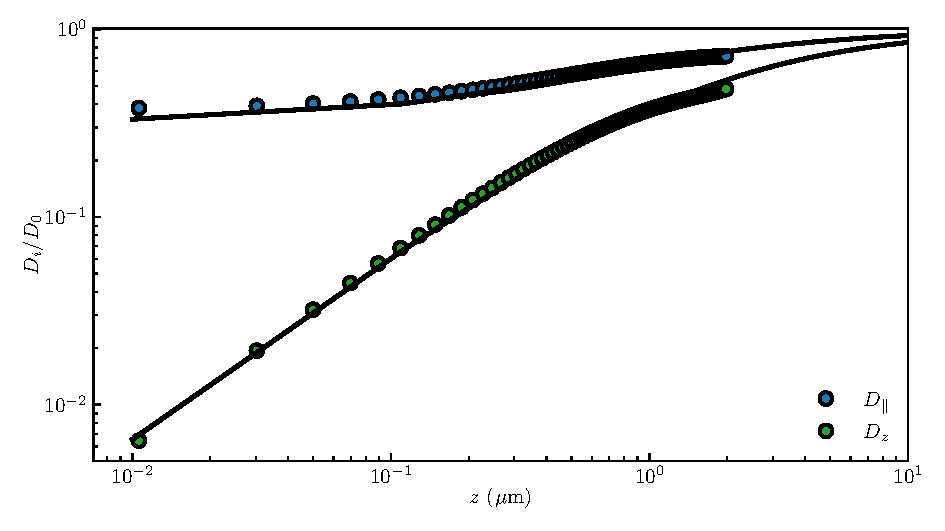
\includegraphics{02_body/chapter3/images/trajctory_analysis/visco.pdf}
	\caption{ Measured local short-term diffusion coefficients $D_i$ of the microparticle, normalized by the bulk value $D_0$, as functions of the distance $z$ to the wall, along both a transverse direction $x$ or $y$ ($D_i=D_\parallel=D_x=D_y$, blue) and the normal direction $z$ ($D_i=D_z$, green) to the wall. The solid lines are the theoretical predictions, $D_{\parallel}(z)=D_0\eta/\eta_{\parallel}(z)$ and $D_z(z)=D_0\eta/\eta_z(z)$, using the local effective viscosities $\eta_{\bot}(z)$ and $\eta_\parallel(z)$ of Eqs.~(\ref{Eq:etaz})~and~(\ref{Eq:etaz}), respectively.~\href{https://github.com/eXpensia/Confined-Brownian-Motion/blob/main/02_body/chapter3/images/trajctory_analysis/graph_ploting.ipynb}{\faGithub}}
	\label{fig.visco}
\end{figure}

\subsubsection{Precise potential inference using multi-fitting technique}
So far, through Figs.~\ref{fig.pdf_exp}-\ref{fig.visco}, we have successively presented the various measured statistical quantities of interest, as well as their fits to corresponding theoretical models. Therein, we have essentially three free physical parameters, $B$, $\ell_\mathrm{B}$, $\ell_\mathrm{D}$, describing the particle and its environment, as well as the \textit{a priori} undetermined location of the $z=0$ origin. These four parameters are actually redundant among the various theoretical models. Therefore, in order to measure them accurately, we in fact perform all the fits simultaneously,
using a Broyden-Fletcher-Goldfarb-Shanno (BFGS) algorithm that is well suited for unconstrained
nonlinear optimization~\cite{dai_convergence_2002}. To do so, we construct a global minimizer:
\begin{equation}
	\chi ^ 2 = \sum _{n=1} ^{N} \chi_n ^ 2\ ,
\end{equation}
where we introduce the minimizer $\chi _n ^2$ of each set $n$ among the $N$ sets of data, defined as:
\begin{equation}
	\chi _n ^2 = \sum _{i=1} ^{M_n} \frac{[y_{ni} - f_n(x_{ni}, \mathbf{b})]^2 }{f_n(x_{ni}\ , \mathbf{b})^2}\ ,
\end{equation}
with $\{x_{ni},y_{ni}\}$ the experimental data of set $n$, $M_n$ the number of experimental data points for set $n$, $f_n$ the model for set $n$, and $\mathbf{b}=(b_1,b_2,...,b_p)$ the $p$ free parameters. In our case, $p=4$, and $\{x_{ni},y_{ni}\}$ represent all the experimental data shown in Figs.\ref{fig.pdf_exp}-\ref{fig.visco}. 

Due to strong dependence of the normal diffusion coefficient $D_z$ with $z$, it is possible to find the wall position with a 10 nm resolution, thus overcoming a drawback of the Lorenz-Mie technique which only provides the axial distance relative to the focus of the objective lens. Besides, the three physical parameters globally extracted from the multifitting procedure are: $B = 4.8 \pm 0.6$, $\ell_\mathrm{D} = 21 \pm 1~ \mathrm{nm} $, and $\ell_\mathrm{B} = 530 \pm 2~ \mathrm{nm}$. Using the particle radius $a = 1.518 \pm 0.006 ~ \mathrm{\mu m}$ calibrated from the preliminary fits of the interference patterns to the Lorenz-Mie scattering function (see section \ref{sec:radius_charac}), and the $\rho_\mathrm{p} = 1050 ~ \mathrm{kg.m^{-3}}$ tabulated bulk density of polystyrene, we would have expected $\ell_\mathrm{B}=559 ~ \mathrm{nm}$ instead, which corresponds to less than $2\,\%$ error, and might be attributed to nanometric offsets, such as \textit{e.g.} the particle and/or wall rugosity. 

\subsubsection{Measuring external forces using the local drifts}
Finally, we investigate the total conservative force $F_z(z)$ acting on the particle along $z$. The first way to measure it is to calculate the gradient of the potential $U$ which is experimentally measured from the position \gls{PDF} giving:


\begin{equation}
	F_z^\mathrm{eq} = -\nabla U = k_\mathrm{B}T \frac{\mathrm{d}}{\mathrm{d} z} \ln (P_\mathrm{eq}) ~,
	\label{Eq.conservative_force}
\end{equation}

where one can use the experimentally measured $P_\mathrm{eq}$ (see Fig.~\ref{fig.pdf_exp}). The results of this method are shown in Fig.~\ref{fig.figure_force_total}. However, it can be interesting to measure the forces using the local drifts as for more complex systems, some non-conservative forces could arise. As the Eq.~(\ref{Eq.conservative_force}) takes only into account to the potential $U$, only conservative forces can be extracted from the measurement of $P_\mathrm{eq}$. Non-conservative forces could be measured by the difference between forces obtained through $P_\mathrm{eq}$ and the local drifts.  


Let us now explain the force measurement from drifts. By averaging the overdamped Langevin of Eq.~(\ref{sde.multipl}) over a fine-enough $z$-binning grid and a short-enough time interval $\Delta t$, one gets in the Itô convention (corresponding to our definition of $\Delta z$):
\begin{equation}
	F_z (z) = 6 \pi \eta_z (z ) a \frac{\langle\Delta z\rangle}{\Delta t} - k_\mathrm{B}T \frac{D_z'(z)}{D_z(z)} \ ,
	\label{stokes}
\end{equation}
where the last term corresponds to the additional contribution due to the non-trivial integration of the multiplicative noise~\cite{volpe_influence_2010,mannella_comment_2011,mannella_ito_2012, sancho_brownian_2011} (see section \ref{sec:spurious}), with the prime denoting the derivative with respect to $z$. From the averaged measured vertical drifts $\langle\Delta z\rangle$, and invoking Eqs.~(\ref{Eq.hindered})~and~(\ref{Eq:etaz_pade}), one can reconstruct $F_z(z)$ from Eq.~(\ref{stokes}), as shown in Fig.~\ref{fig.figure_force_total}. We stress that the statistical error on the force measurement is comparable to the thermal-noise limit~\cite{liu_subfemtonewton_2016}: 
\begin{equation}
	\label{tnl}
	\Delta F=\sqrt{24\pi k_{\mathrm{B}}T \eta_z(z) a/ \tau_{\textrm{box}}(z)}\ ,
\end{equation}
where $\tau_{\textrm{box}}(z)$ is the total time spent by the particle in the corresponding box of the $z$-binning grid. To corroborate these measurements, we invoke Eq.~(\ref{Eq:PDF}) and express the total conservative force $F_z(z)=-U'(z)$ acting on the particle along $z$:
\begin{equation}
	\displaystyle F_z(z) =  k_{\mathrm{B}}T\left(\frac{B}{\ell_\mathrm{D}} \textrm{e}^{-\frac{z}{\ell_\mathrm{D}}} - \frac{1}{\ell_\mathrm{B}}\right)\ .
	\label{Eq:Force}
\end{equation} 
Using the physical parameters extracted from the above multifitting procedure, we plot Eq.~(\ref{Eq:Force}) in Fig.~\ref{fig.figure_force_total}. The agreement with the data is excellent, thus showing the robustness of the force measurement. In particular, we can measure forces down to a distance of $40$~nm from the surface. Besides, far from the wall, we are able to resolve the actual buoyant weight $F_{\textrm{g}} =- 7  \pm 4 ~ \mathrm{fN}$ of the particle. This demonstrates that we reach the femtoNewton resolution, and that this resolution is solely limited by thermal noise.
\begin{figure}[H]
	\centering
	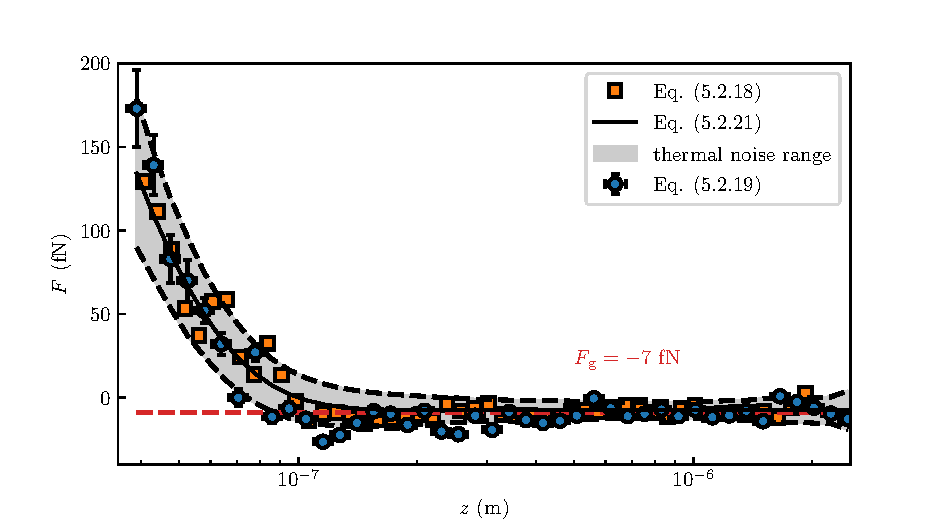
\includegraphics{02_body/chapter3/images/trajctory_analysis/figure_force_total.pdf}
	\caption{Total normal conservative force $F_z$ exerted on the particle as a function of the distance $z$ to the wall, reconstructed from Eq.~(\ref{stokes}), using Eq.~(\ref{Eq:etaz_pade}) for the circles and Eq.~(\ref{Eq.conservative_force}) for the squares. The solid line corresponds to Eq.~(\ref{Eq:Force}), with $B=4.8$, $\ell_{\mathrm{D}}=21\,\mathrm{nm}$ and $\ell_{\mathrm{B}}=530\,\mathrm{nm}$. The black dashed lines and gray area indicate the amplitude of the thermal noise computed from Eq.~(\ref{tnl}). The horizontal red dashed line indicates the buoyant weight $F_{\textrm{g}}=-7$~fN of the particle.~\href{https://github.com/eXpensia/Confined-Brownian-Motion/blob/main/02_body/chapter3/images/trajctory_analysis/measure_force_experimental.ipynb}{\faGithub}}
	\label{fig.figure_force_total}
\end{figure}

\subsection{Conclusion}

In this section we have covered the physics we need to take into account when considering confined Brownian motion. We first detailed the gravitational and DLVO interactions to detail the Gibbs-Boltzmann distribution. Then, we detail the space-varying damping due to the hydrodynamic interactions between the wall and the particle. The damping which is now space-varying in the Langevin induces a non-trivial integration of the Langevin force, which induces the appearance of a spurious drift term in the Fokker-Planck equation. We then present a method that permits to estimate how the simulation time-step should be selected, then we show that the spurious drift term is needed to be taken into account to recover the correct equilibrium distribution.

In a second part, we present a multi-scale statistical analysis for the problem of freely diffusing individual colloids near a rigid wall. Combining the equilibrium distribution in position, time-dependent non-Gaussian statistics for the spatial displacements, a novel method to infer local diffusion coefficients, and a multifitting procedure, allowed us to reduce drastically the measurement uncertainties and reach the nanoscale and thermal-noise-limited femtoNewton spatial and force resolutions, respectively.



